\documentclass[10pt,journal,compsoc]{IEEEtran}
\usepackage{enumerate}
\usepackage{cite}
\usepackage{amsmath}
\interdisplaylinepenalty=2500
\usepackage{algorithm}
\usepackage{algorithmic}
\usepackage{graphicx}
\usepackage{multirow}
\usepackage{subfigure}
\usepackage{amssymb}
\usepackage[normalem]{ulem}
\usepackage{color}
\usepackage{ulem}
\hyphenation{op-tical net-works semi-conduc-tor}


\begin{document}

\title{Dynamic Random Testing of Web Services: \\ A Methodology and Evaluation}


\author{Chang-ai~Sun,~\IEEEmembership{Senior Member,~IEEE,}
        Hepeng~Dai,
        Guan~Wang,
        Dave~Towey,~\IEEEmembership{Member,~IEEE,}
        Tsong Yueh~Chen,~\IEEEmembership{Member,~IEEE,}
        and~Kai-Yuan~Cai,~\IEEEmembership{Member,~IEEE,}
\thanks{A preliminary version of this paper was presented at the 36th Annual IEEE Computer Software and Applications Conference (COMPSAC 2012)~\cite{sun2012towards}.}
\thanks{C.-A. Sun, H. Dai, and G. Wang are with the School of Computer and Communication Engineering, University of Science and Technology Beijing, Beijing 100083, China. E-mail: casun@ustb.edu.cn.}% <-this % stops a space
\thanks{D. Towey is with the School of Computer Science, University of Nottingham Ningbo China, Ningbo 315100, China. E-mail: dave.towey@nottingham.edu.cn}
\thanks{K.-Y. Cai is with the School of Automation Science and Electrical Engineering, Beihang University, Beijing 100191, China. E-mail: kycai@buaa.edu.cn.}% <-this % stops a
\thanks{T.Y. Chen is with the Department of Computer Science and Software Engineering, Swinburne University of Technology, Hawthorn VIC 3122, Australia. Email: tychen@swin.edu.au.}
}


\markboth{IEEE TRANSACTIONS ON SERVICES COMPUTING,~submitted}%
{Sun \MakeLowercase{\textit{Sun et al.}}: An Empirical Study on Dynamic Random Testing of Web Services: A Methodology and Evaluation}


\IEEEtitleabstractindextext{
\begin{abstract}
  In recent years, Service Oriented Architecture (SOA) has been increasingly adopted to develop distributed applications in the context of the Internet. To develop reliable SOA-based applications, an important issue is how to ensure the quality of web services. In this paper, we propose a dynamic random testing (DRT) technique for web services, which is an improvement over the widely-practiced random testing (RT)~and partition testing (PT). We examine key issues when adapting DRT to the context of SOA, including a framework, guidelines for parameter settings, and a prototype for such an adaptation. Empirical studies are reported where DRT is used to test three real-life web services, and mutation analysis is employed to measure the effectiveness. Our experimental results show that, compared with the two baseline techniques, RT and Random Partition Testing (RPT), DRT demonstrates higher fault-detection effectiveness with a lower test case selection overhead. Furthermore, the theoretical guidelines of parameter setting for DRT are confirmed to be effective. The proposed DRT and the prototype provide an effective and efficient approach for testing web services.
\end{abstract}

\begin{IEEEkeywords}
Software Testing, Random Testing, Dynamic Random Testing, Web Service, Service Oriented Architecture.
\end{IEEEkeywords}}

\maketitle

\IEEEdisplaynontitleabstractindextext


\IEEEpeerreviewmaketitle


\section{Introduction}
\label{sec:introduction}

\IEEEPARstart{S}{ervice} oriented architecture (SOA)~\cite{papazoglou2008service} defines a loosely coupled, standards-based, service-oriented application development paradigm in the context of the Internet.
Within SOA, three key roles are defined:
service providers (who  develop and own services);
service requestors (who consume or invoke services); and
a service registry (that registers services from providers and returns services to requestors).
Applications are built upon services that present functionalities through publishing their interfaces in appropriate repositories, abstracting away from the underlying implementation.
Published interfaces may be searched by other services or users, and then invoked.
Web services are the realization of SOA based on open standards and infrastructures~\cite{sun2011transaction}.
Ensuring the reliability of SOA-based applications can become critical when such applications implement important business processes.

Software testing is a practical method for ensuring the quality and reliability of software.
However, some SOA features can pose challenges for the testing of web services~\cite{bartolini2009whitening, canfora}.
For instance, service requestors often do not have access to the source code of web services which are published and owned by another organization, and, consequently, it is not possible to use white-box testing techniques.
Testers may, therefore, naturally turn to black-box testing techniques.

Random Testing (RT)~\cite{Hamlet02} is one of the most widely-practiced black-box testing techniques.
Because test cases in RT are randomly selected from the input domain (which refers to the set of all possible inputs of the software under test), it can be easy to implement.
Nevertheless, because RT does not make use of any information about the software under test (SUT), or the test history, it may be inefficient in some situations.
In recent years, many efforts have been made to improve to RT in different ways~\cite{cai2009random, chen2010adaptive, Cai07}.
Adaptive random testing (ART)~\cite{chen2010adaptive, chen2009adaptive, chen2013code, chen2018test}, for example, has been proposed to improve RT by attempting to have a more diverse distribution of test cases in the input domain.

In contrast to RT, partition testing (PT) attempts to generate test cases in a more ``systematic'' way, aiming to use fewer test cases to reveal more faults.
When conducting PT, the input domain of the SUT is divided into disjoint partitions, with test cases then selected from each and every one.
Each partition is expected to have a certain degree of homogeneity---test cases in the same partition should have similar software execution behavior.
Ideally, a partition should also be homogeneous in fault detection:
If one input can reveal a fault, then all other inputs in the same partition should also be able to reveal a fault.

RT and PT are based on different intuitions, and each have their own advantages and disadvantages.
Because it is likely that they can be complementary to each other, detecting different faults, it is intuitively appealing to investigate the their integration.

In traditional RPT \cite{cai2009random}, the partitions and corresponding test profiles remain constant throughout testing, which may not be the best strategy.
Independent researchers have observed that fault-revealing inputs tend to cluster into ``continuous regions''~\cite{Ammann88, Finelli91}---there is similarity in the execution behavior of neighboring software inputs.
Based on software cybernetics, Cai et al. proposed dynamic random testing (DRT)~\cite{cai2009random}, aiming to improve on both RT and RPT.

In practice, web services have usually been tested by the service providers, and simple or easy-to-test faults have been removed, meaning that the remaining faults are normally hard to detect.
For ensuring a higher reliability of the web services, a simple RT strategy may not be an appropriate technique~\cite{li2014two}, especially when the scale is large, or there are some stubborn faults.

In this paper, we present a dynamic random testing (DRT) approach for web services, as an enhanced version of RT that is an adaptation of DRT to the context of SOA.
We examine key issues of such an adaption, and conduct empirical studies to evaluate the feasibility and effectiveness of the proposed DRT, with the experimental results showing DRT outperforms RT in terms of fault detection efficiency.
The contributions of this work include:

\begin{itemize}
  \item
  We develop an effective and efficient testing method for web services.
  This includes a DRT framework that addresses key issues for testing web services, and a prototype that partly automates the framework.
  \item
  We evaluate the performance of DRT through a series of empirical studies on three real web services.
  These studies show that DRT has significantly higher fault-detection efficiency than RT and RPT. That is, to detect a given number of faults, DRT uses less time and fewer test cases than RT and RPT.
  \item
  We provide guidelines for the DRT parameter settings, supported by theoretical analysis, and validated by the empirical studies.
\end{itemize}

The rest of this paper is organized as follows.
Section~\ref{sec:background} introduces the underlying concepts for DRT, web services and mutation analysis.
Section~\ref{sec:DRTforwebserivce} presents the DRT framework for web services, guidelines for its parameter settings, and a prototype that partially automates DRT.
Section~\ref{sec:empiricalstudy} describes an empirical study where the proposed DRT is used to test three real-life web services, the results of which are summarized in Section~\ref{sec:results}.
Section~\ref{sec:relatedwork} discusses related work and Section~\ref{sec:conclusion} concludes the paper.

\section{Background}
\label{sec:background}

In this section, we present some of the underlying concepts for DRT, web services, and mutation analysis.

\subsection{Dynamic Random Testing (DRT)}
\label{sec:DRTStrategy}

DRT combines RT and PT [31], with the goal of benefitting from the advantages of both.
Given a test suite \emph{TS} classified into $m$ partitions (denoted $s_1, s_2, \ldots, s_m$),  suppose that a test case from $s_i$ ($i = 1, 2, \ldots, m$) is selected and executed.
If this test case reveals a fault, $\forall j = 1, 2, \ldots, m$ and $j \neq i$, we then set

\begin{equation}
\label{eq:DRThitJ}
p'_j =
\begin{cases}
p_j - \displaystyle\frac{\varepsilon}{m-1} & \text{if } p_j \geq \displaystyle\frac{\varepsilon}{m-1} \\
0 & \text{if } p_j < \displaystyle\frac{\varepsilon}{m-1}
\end{cases},
\end{equation}
where $\varepsilon$ is a probability adjusting factor, and then

\begin{equation}
\label{eq:DRThitI}
  p'_i = 1 - \sum_{\substack{j = 1 \\ j \neq i}}^m p'_j.
\end{equation}

Alternatively, if the test case does not reveal a fault, we set

\begin{equation}
\label{eq:DRTmissI}
p'_i =
\begin{cases}
p_i - \varepsilon & \text{if } p_i \geq \varepsilon \\
0 & \text{if } p_i < \varepsilon
\end{cases},
\end{equation}

and then for $\forall j = 1, 2, \ldots, m$ and $j \neq i$, we set

\begin{equation}
\label{eq:DRTmissJ}
p'_j =
\begin{cases}
p_j + \displaystyle\frac{\varepsilon}{m-1} & \text{if } p_i \geq \varepsilon \\
p_j + \displaystyle\frac{p'_i}{m-1} & \text{if } p_i < \varepsilon
\end{cases}.
\end{equation}

Algorithm \ref{alg:DRT} describes DRT.
In DRT, the first test case is taken from a partition that has been randomly selected according to the initial probability profile $\{p_1, p_2, \ldots, p_m\}$ (Lines 2 and 3 in Algorithm~\ref{alg:DRT}).
After each test case execution, the testing profile $\{ \left \langle s_1,p_1 \right \rangle, \left \langle s_2,p_2 \right \rangle, \ldots, \left \langle s_m,p_m \right \rangle\}$ is updated by changing the values of $p_i$:
If a fault is revealed, Formulas~\ref{eq:DRThitJ} and~\ref{eq:DRThitI} are used;
otherwise, Formulas~\ref{eq:DRTmissI} and~\ref{eq:DRTmissJ} are used.
The updated testing profile is then used to guide the random selection of the next test case (Line 8).
This process is repeated until a termination condition is satisfied (Line 1).
Examples of possible termination conditions include:
 ``testing resources have been exhausted'';
 ``a certain number of test cases have been executed''; and
 ``a certain number of faults have been detected".

\begin{algorithm}
    \caption{DRT}
    \label{alg:DRT}
    \begin{algorithmic}[1]
        \renewcommand{\algorithmicrequire}{\textbf{Input:}} %ʹ��ԭ���������ж��������\REQUIRE ��\ENSURE��ʾΪInput:��Output:
	    \renewcommand{\algorithmicensure}{\textbf{Output:}}
        \renewcommand{\algorithmicendwhile}{\algorithmicend\_\algorithmicwhile}
		\renewcommand{\algorithmicendfor}{\algorithmicend\_\algorithmicfor}
		\renewcommand{\algorithmicendif}{\algorithmicend\_\algorithmicif}
		\renewcommand{\algorithmicthen}{}
		\renewcommand{\algorithmicdo}{}
        \REQUIRE $\varepsilon, p_1, p_2, \ldots, p_m$
        \WHILE {termination condition is not satisfied}
        \STATE Select a partition $s_i$ according to the testing profile $\{ \left \langle s_1,p_1 \right \rangle, \left \langle s_2,p_2 \right \rangle, \ldots, \left \langle s_m,p_m \right \rangle\}$.
        \STATE Select a test case $t$ from $s_i$.
        \STATE Test the software using $t$.
        \IF {a fault is revealed by $t$}
        \STATE Update $p_j$ ($j = 1, 2, \ldots, m$ and $j \neq i$) and $p_i$ according to Formulas~\ref{eq:DRThitJ} and~\ref{eq:DRThitI}.
        \ELSE
        \STATE Update $p_j$ ($j = 1, 2, \ldots, m$ and $j \neq i$) and $p_i$ according to Formulas~\ref{eq:DRTmissI} and~\ref{eq:DRTmissJ}.
        \ENDIF
        \ENDWHILE
    \end{algorithmic}
\end{algorithm}

As can be seen from Formulas~\ref{eq:DRThitJ} to~\ref{eq:DRTmissJ},  updating the testing profile involves $m$ simple calculations, thus requiring a constant time.
Furthermore, the selection of partition $s_i$, and subsequent selection and execution of the test case, all involve a constant time.
The execution time for one iteration of DRT is thus a constant, and therefore the overall time complexity for DRT to select $n$ test cases is $O(m \cdot n)$.

\subsection{Web Services}

A web service is a platform-independent, loosely coupled, self-contained, programmable, web-enabled application that can be described, published, discovered, coordinated and configured using XML artifacts for the purpose of developing distributed interoperable applications~\cite{papazoglou2008service}.
A web service consists of a description (usually specified in WSDL) and implementation (written in any programming language).
Web services present their functionalities through published interfaces, and are usually deployed in a service container.
Invocation of a web service requires analysis of the input message in its WSDL, test data generation based on its input parameters, and wrapping of test data in a SOAP message.

A web service is a basic component of SOA software, and, accordingly, the reliability of such SOA software depends heavily on the quality of the component web services.
While testing is an obvious potential activity to help assuring the quality of web services, due to the unique features of SOA, web service testing can be more challenging than traditional software testing \cite{canfora}.
Some of these features include:
\begin{itemize}
  \item
  \emph{Lack of access to service implementation:}
  Normally, web service owners will not make source code of their web services accessible.
  Typically, service users only have access to the service interface defined in a WSDL file, which means that white-box testing approaches are not possible.
  \item
  \emph{Incomplete documentation or specification:}
  A service provider may only offer an incomplete or inaccurate description of a service's functional and non-functional behavior.
  This makes it difficult to decide whether or not a test passes, especially when details about behavior or restrictions on implementations are missing \cite{sun2018constraint}.
  \item
  \emph{Lack of control:}
  Unlike traditional software testing where testers can control the execution of software under test, there is usually no opportunity to intervene in the execution of the web service under test, which is often deployed in a remote service container.

  \item
  \emph{Side effects caused by testing:}
  A large number of tests may introduce an additional communication load, and hence impact on the performance of the web service under test.
  This suggests that the number of tests should be kept as low as possible \cite{sunreview}.
\end{itemize}

\section{DRT for Web Services}
\label{sec:DRTforwebserivce}

In this section, we describe a framework for applying DRT to web services, discuss guidelines for DRT's parameter settings, and present a prototype that partially automates  DRT for web services.

\subsection{Framework}
\label{sec:framework}

Considering the principle of DRT and the features of web services, we propose a DRT for web services framework, as illustrated in Figure~\ref{fig:frame}.
In the figure, the DRT components are inside the box, and the web services under test are located outside.
Interactions between DRT components and the web services are depicted in the framework.
We next discuss the individual framework components.

\begin{figure}[]
  \centering
  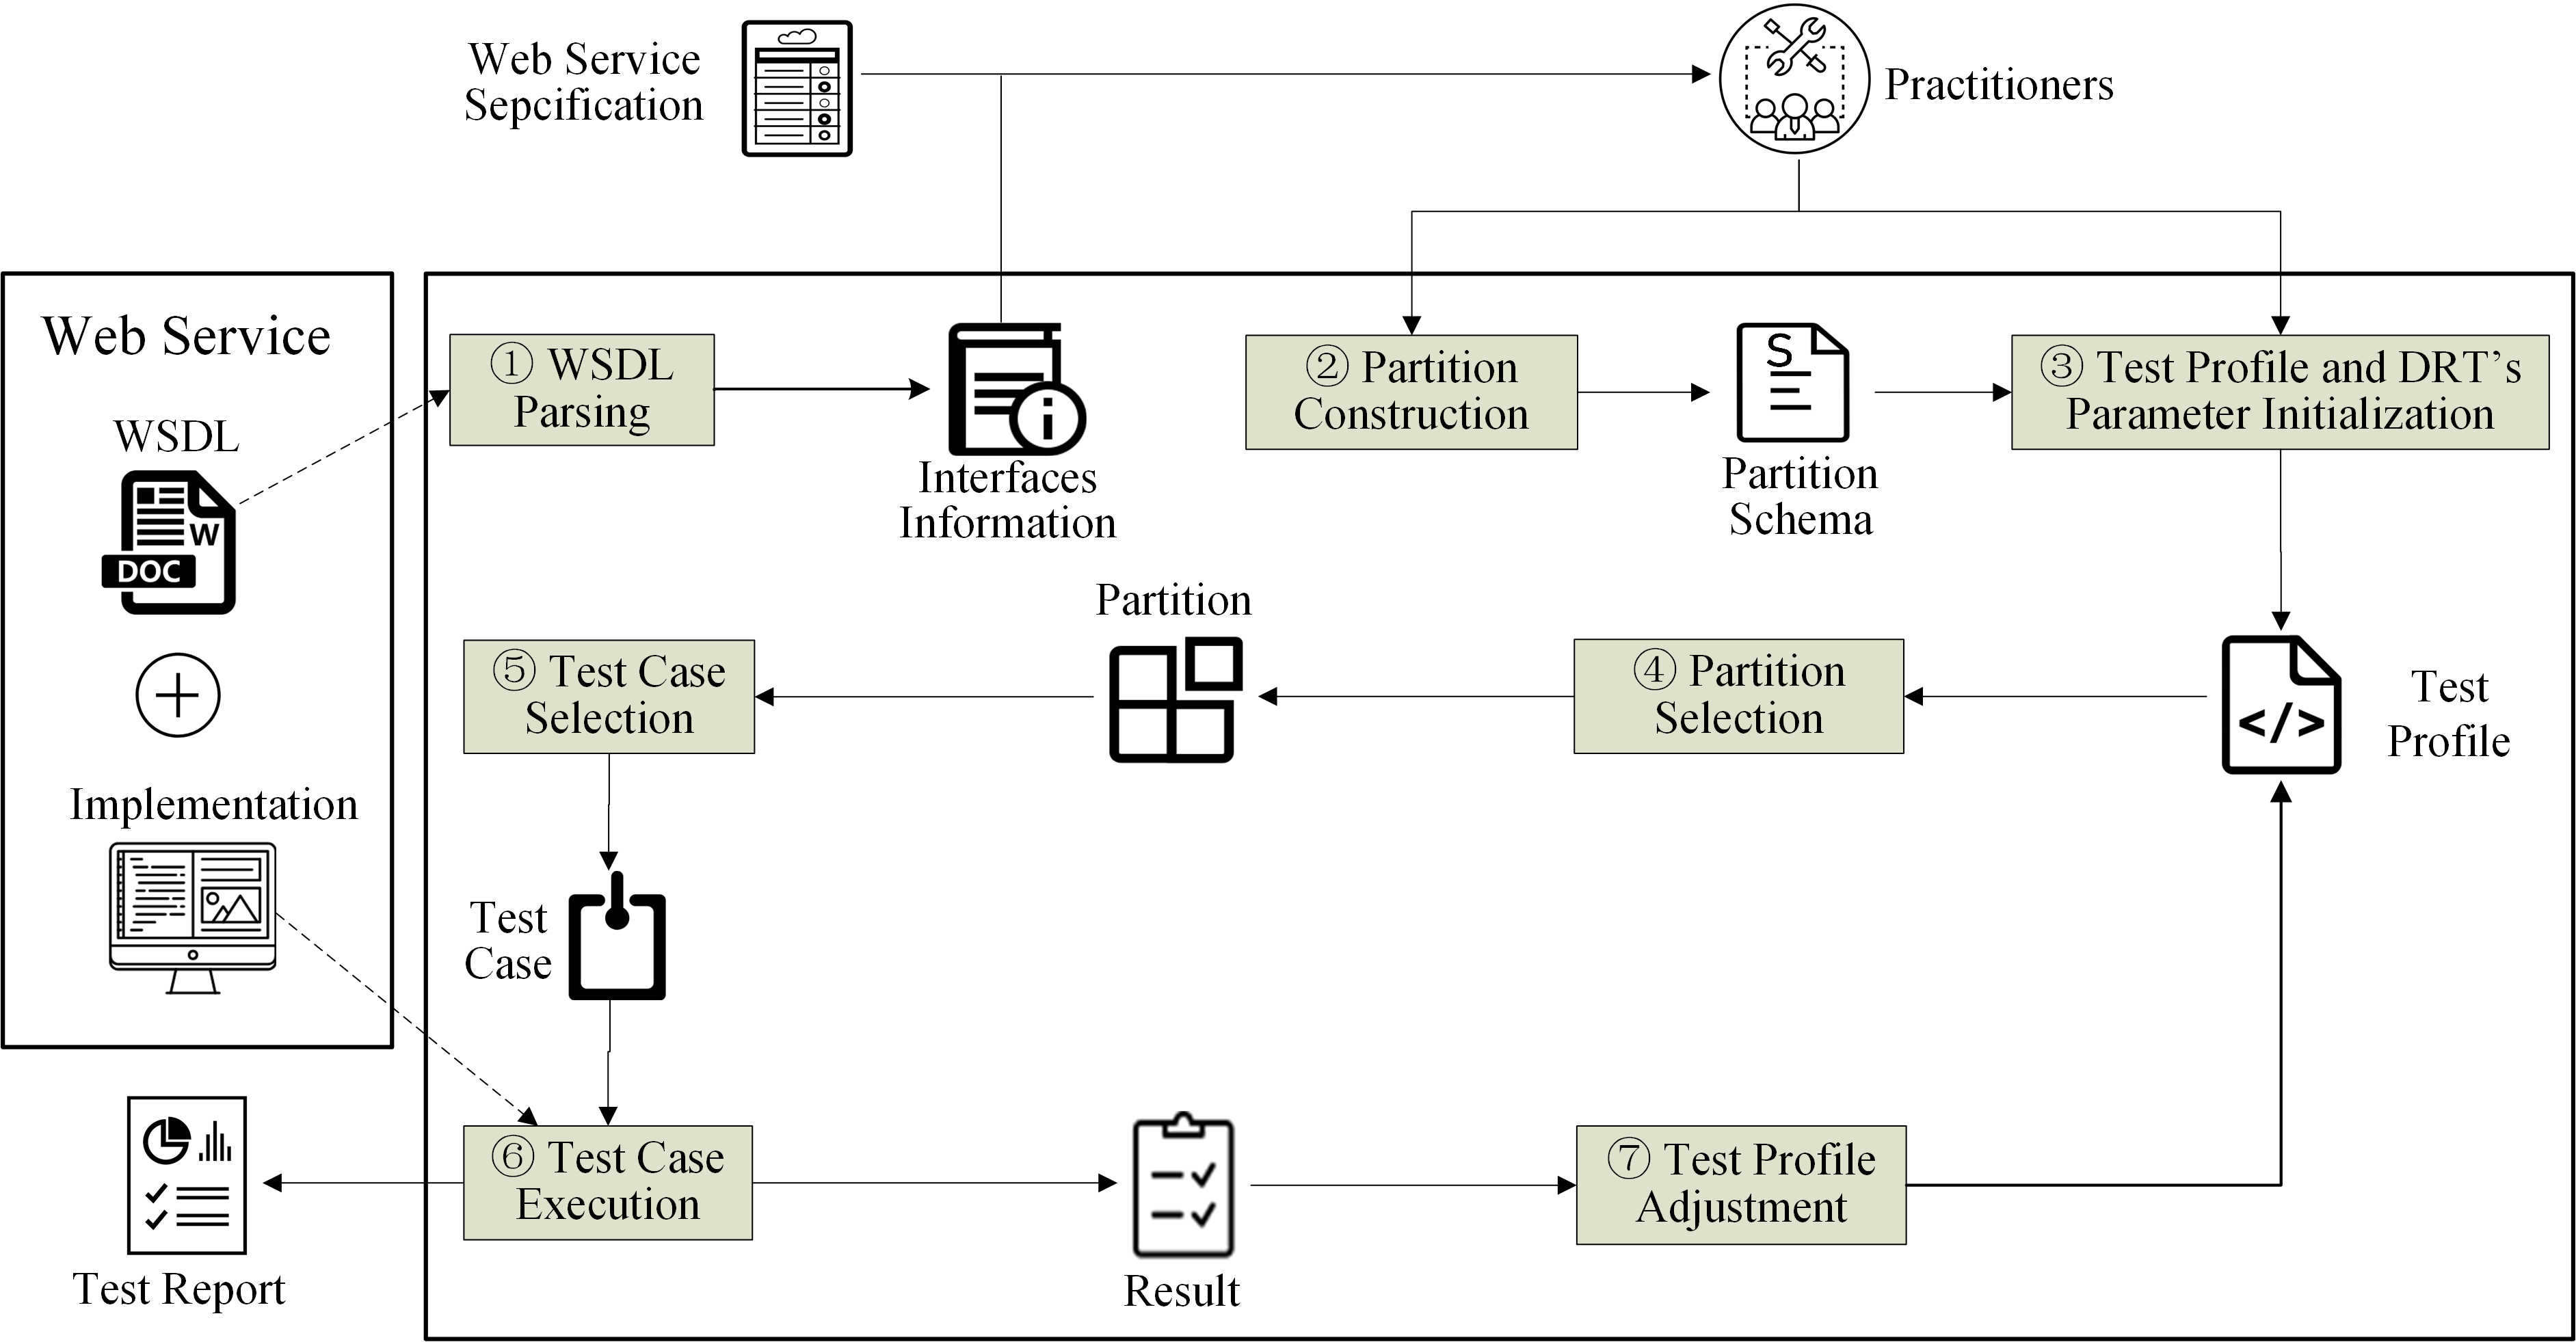
\includegraphics[width = 0.5\textwidth]{fig//framework.png}
  \caption{DRT for web services framework}
  \label{fig:frame}
\end{figure}

\begin{enumerate}[1]
  \item
  \emph{WSDL Parsing}.
  Web services are composed of services and the relevant WSDL documents.
  By parsing the WSDL document, we can get the input information for each operation in the services.
  This includes the number of parameters, their names and types, and any additional requirements that they may have.

  \item
  \emph{Partition Construction}.
  Partition testing (PT) refers to a class of testing techniques that break the input domain into a number of partitions~\cite{weyuker1991analyzing}.
  Because DRT is a black-box testing technique, combining RT and PT, the PT approaches used are at the specification level.
  Various approaches and principles for achieving convenient and effective partitions have been discussed in the literature~\cite{weyuker1991analyzing, cai2005partition, chen1994relationship, chen1996expected}.
  The input domain of the web service under test (WSUT) can be partitioned based on the WSUT specifications and the parsed parameters.
  Once partitioned, testers can assign probability distributions to the partitions as an initial testing profile.
  This initial testing profile can be assigned in different ways, including using a uniform probability distribution, or one that sets probabilities according to the importance of the partition:
  For example, a partition within which faults were previously detected should be given higher priority.

  \item
  \emph{Partition Selection}.
  DRT randomly selects a partition $s_i$ according to the test profile.

  \item
  \emph{Test Case Generation}.
  Given the selected partition $s_i$, a test case is then randomly and independently generated within $s_i$.
  Because the WSDL document has been parsed, generation of test cases can be automated.

  \item
  \emph{Test Case Execution}.
  The relevant DRT component receives the generated test case, converts it into an input message, invokes the web service(s) through the SOAP protocol, and intercepts the test results (from the output message).

  \item
  \emph{Test Profile Adjustment}.
  Upon completion of each test, its pass or fail status is determined by comparing the actual and expected results (with pass if both are the same).
  The pass or fail status is then used to adjust the (partition) probability distribution accordingly.
  Situations where determination of the test outcome status is not possible (i.e. in the presence of the oracle problem~\cite{weyuker1982testing, barr2015oracle, patel2018mapping}) may potentially be addressed using metamorphic testing~\cite{sun2011}.
\end{enumerate}

Generally speaking, DRT test case generation is both in accordance with the probability distribution (for selection of the relevant partition), and with the principles of RT, taking advantage of the ease of RT and the effectiveness of PT.
Furthermore, many of the DRT for web services framework components can be automated.
To make DRT for web services more efficient and practical, we developed a prototype that will be described in Section~\ref{sec:prototype}.

\subsection{Guidelines for Parameter Setting}
\label{sec:relation}

Our previous work~\cite{sun2012towards} found that the DRT performance depends on the number of partitions and the parameter $\varepsilon$.
We next explore these impacts through a theoretical analysis, which, to be mathematically tractable, has the following assumptions:

\begin{enumerate}[1]
  \item
  The failure rate $\theta_i$ of each partition $s_i$ ($i = 1, 2, \ldots, m$, and $m > 1$) is unknown, but can be estimated.

  \item
  Each failure rate~$\theta_i$ ($i = 1, 2, \ldots, m$, and $m > 1$) remains unchanged throughout the testing process (faults are not removed after their detection).

  \item
  Test cases are selected with replacement, which means that same test cases may be selected more than once.
\end{enumerate}

A principle of the DRT strategy is to increase the selection probabilities (by amount $\varepsilon$) of partitions with larger failure rates.
In addition to the impact of the parameter $\varepsilon$, the number of partitions also influences the speed of updating the testing profile (Formulas \ref{eq:DRThitJ} to \ref{eq:DRTmissJ}).
Therefore, for a given number of partitions, we are interested in investigating what values of $\varepsilon$ yield the best DRT performance.

Letting $\theta_M$ denote the maximum failure rate, and $s_M$ denote partitions with that failure rate, then $p_i^n$ denotes the probability of executing the $n^{th}$ test case from partition $s_i$.
As testing proceeds, the probability $p_M$ of partition $s_M$ being selected is expected to increase:
\begin{equation}
    \label{eq:exception}
    p_M^{n + 1} > p_M^{n}
\end{equation}

Initially, the testing profile is
$\{ \left \langle s_1,p_1^0 \right \rangle, \left \langle s_2,p_2^0 \right \rangle, \ldots, \left \langle s_m,p_m^0 \right \rangle\}$,
which, after $n$ test cases have been executed,  is then updated to
$\{ \left \langle s_1,p_1^n \right \rangle, \left \langle s_2,p_2^n \right \rangle, \ldots, \left \langle s_m,p_m^n \right \rangle\}$.
During the testing process, $p_i^n$ is increased or decreased by the value $\varepsilon$, which is relatively small (set to $0.05$ in previous studies \cite{Lv2011,li2015}).
Because the initial $p_i^0$ is larger than $\varepsilon$, and the adjustment of $p_i$ is relatively small (Formulas~\ref{eq:DRThitJ} to~\ref{eq:DRTmissJ}), the following two situations are rare, and thus not considered here:
$p_i < \varepsilon / (m - 1)$ or
$p_i < \varepsilon$ ($i = 1, 2, \ldots, m$).

To explore the relationship between $p_i^{n + 1}$ and $p_i^{n}$, we calculate the conditional probability, $p(i|\delta)$, of the following four situations (denoted $\delta_1, \delta_2, \delta_3$, and $\delta_4$, respectively):

\begin{enumerate}[ {Situation} 1 ($\delta_1$):]
  \item
  \textbf{If $t_{n} \notin s_i$ and a fault is detected by $t_n$}, then $p(i|\delta_1)$ is calculated according to Formula \ref{eq:DRThitJ}:
    $$p(i|\delta_1) = \sum_{i \neq j}\theta_j(p_i^n - \displaystyle\frac{\varepsilon}{m - 1}).$$

  \item
  \textbf{If $t_{n} \in s_i$ and a fault is detected by $t_n$}, then $p(i|\delta_2)$ is calculated according to Formula \ref{eq:DRThitI}:
    $$p(i|\delta_2) = \theta_i(p_i^n + \varepsilon).$$

  \item
  \textbf{If $t_{n} \in s_i$ and no fault is detected by $t_n$}, then $p(i|\delta_3)$ is calculated according to Formula \ref{eq:DRTmissI}:
    $$p(i|\delta_3) = (1 - \theta_i)(p_i^n - \varepsilon).$$

  \item
  \textbf{If $t_{n} \notin s_i$ and no fault is detected by $t_n$}, then $p(i|\delta_4)$ is calculated according to Formula \ref{eq:DRTmissJ}:
    $$p(i|\delta_4) = \sum_{i \neq j}(1 - \theta_j)(p_i^n + \displaystyle\frac{\varepsilon}{m - 1}).$$
\end{enumerate}

Therefore, $p_i^{n + 1}$ for all cases together is:

\begin{equation}
    \label{eq:7}
    \begin{split}
    p_i^{n + 1} = &p_i^n\theta_i(p_i^n + \varepsilon) + p_i^n(1-\theta_i)(p_i^n - \varepsilon)\\
    &+ \sum_{j \neq i}p_j^n\theta_j(p_i^n - \displaystyle \frac{\varepsilon}{m- 1})\\
    &+ \sum_{j \neq i}p_j^n(1 - \theta_j)(p_i^n + \displaystyle\frac{\varepsilon}{m - 1})\\
    =&(p_i^n)^2\theta_i + p_i^n\theta_i\varepsilon + (p_i^n)^2 - p_i^n\varepsilon - (p_i^n)^2\theta_i + p_i^n\theta_i\varepsilon\\
    & + (p_i^n - \displaystyle\frac{\varepsilon}{m - 1})\sum_{j \neq i}p_j^n\theta_j + (p_i^n + \displaystyle\frac{\varepsilon}{m - 1})\sum_{j \neq i}p_j^n\\
    &- (p_i^n + \displaystyle\frac{\varepsilon}{m - 1})\sum_{j \neq i}p_j^n\theta_j\\
    =&(p_i^n)^2 + 2p_i^n\theta_i\varepsilon - p_i^n\varepsilon + (p_i^n - \displaystyle\frac{\varepsilon}{m - 1} - p_i^n \\
    &- \displaystyle\frac{\varepsilon}{m - 1})\sum_{j \neq i}p_j^n\theta_j + (p_i^n + \displaystyle\frac{\varepsilon}{m - 1})(1 - p_i^n)\\
    =&p_i^n + (p_i^n)^2 - (p_i^n)^2 + 2p_i^n\theta_i\varepsilon - p_i^n\varepsilon + \displaystyle\frac{\varepsilon}{m - 1} - \\
    &\displaystyle\frac{\varepsilon}{m - 1}p_i^n - \displaystyle\frac{2\varepsilon}{m - 1}\sum_{j \neq i}p_j^n\theta_j\\
    =&p_i^n + \displaystyle\frac{\varepsilon}{m - 1}(2p_i^n\theta_im - p_i^nm - 2p_i^n\theta_i + 1 )\\
    &- \displaystyle\frac{2\varepsilon}{m-1}\sum_{j \neq i}p_j^n\theta_j\\
    =&p_i^n + Y_i^n,
    \end{split}
\end{equation}
where
\begin{equation}
    \begin{split}
    \label{eq:yi}
    Y_i^n = &\displaystyle\frac{\varepsilon}{m - 1}(2p_i^n\theta_im - p_i^nm - 2p_i^n\theta_i + 1 )\\
             &- \displaystyle\frac{2\varepsilon}{m-1}\sum_{j \neq i}p_j^n\theta_j.
    \end{split}
 \end{equation}

From Formula~\ref{eq:yi}, we have:
 \begin{equation}
    \begin{split}
    \label{eq:26}
    Y_M^n - Y_i^n = &\displaystyle\frac{\varepsilon}{m - 1}(2p_M^n\theta_Mm - p_M^nm - 2p_M^n\theta_M + 1)\\
    & - \displaystyle\frac{2\varepsilon}{m - 1}\sum_{j \neq M}p_j^n\theta_j - \displaystyle\frac{\varepsilon}{m - 1}(2p_i^n\theta_im - p_i^nm\\
    & - 2p_i^n\theta_i + 1) + \displaystyle\frac{2\varepsilon}{m - 1}\sum_{j \neq i}p_j^n\theta_j \\
    =&\displaystyle\frac{\varepsilon}{m - 1}(2m(p_M^n\theta_M - p_i^n\theta_i) - m(p_M^n - p_i^n) -\\
    & 2(p_M^n\theta_M - p_i^n\theta_i)) - \sum_{j \neq M}p_j^n\theta_j + \sum_{j \neq i}p_j^n\theta_j    \\
    =& \displaystyle\frac{2\varepsilon}{m - 1}(m(p_M^n\theta_M - p_i^n\theta_i) - \displaystyle\frac{m(p_M^n - p_i^n)}{2} - \\
    &(p_M^n\theta_M - p_i^n\theta_i)) + \displaystyle\frac{2\varepsilon}{m-1}(p_M^n\theta_M - p_i^n\theta_i)\\
    =&\displaystyle\frac{2\varepsilon}{m - 1}(m(p_M^n\theta_M - p_i^n\theta_i) - \displaystyle\frac{m(p_M^n - p_i^n)}{2}).
    \end{split}
\end{equation}

Before presenting the final guidelines, we need the following lemma.
\newtheorem{lem}{Lemma}
\label{Lemma}
\begin{lem}
  If $p_i^{n} - p_M^{n} > 2(p_i^{n}\theta_i - p_M^{n}\theta_M)$, then $p_M^{n + 1} > p_M^{n}$.
\end{lem}
\begin{IEEEproof}
The condition $p_i^{n} - p_M^{n} > 2(p_i^{n}\theta_i - p_M^{n}\theta_M)$ can be equivalently expressed as:
\begin{equation}
  \label{lemma:proof1}
\displaystyle\frac{p_M^n - p_i^n}{2} < p_M^{n}\theta_M - p_i^{n}\theta_i.
\end{equation}

From Formula~\ref{lemma:proof1},  $(p_M^{n}\theta_M - p_i^{n}\theta_i) - \displaystyle\frac{p_M^n - p_i^n}{2} > 0$, and because $0 < \varepsilon < 1$, and $m > 1$,  therefore:
\begin{equation}
  \label{lemma:proof2}
\displaystyle\frac{2m\varepsilon}{m - 1}((p_M^{n}\theta_M - p_i^{n}\theta_i) - \displaystyle\frac{p_M^n - p_i^n}{2}) > 0.
\end{equation}

Furthermore:
\begin{equation}
  \label{lemma:proof3}
\displaystyle\frac{2\varepsilon}{m - 1}(m(p_M^{n}\theta_M - p_i^{n}\theta_i) - \displaystyle\frac{m(p_M^n - p_i^n)}{2}) > 0.
\end{equation}

According to Formulas \ref{lemma:proof3} and \ref{eq:26},
if $p_i^{n} - p_M^{n} > 2(p_i{n}\theta_i - p_M^{n}\theta_M)$, then
$Y_M^n - Y_i^n > 0$.

Also, because
$\sum_{i=1}^mp_i^{n + 1} = 1$, and
$\sum_{i=1}^mp_i^{n} = 1$, therefore
$Y_M^n >0$, and thus
$\sum_{i=1}^mY_i^n = 0$.

According to Formula~\ref{eq:7},
$p_M^{n + 1} = p_M^n + Y_M^n$.
Because $Y_M^n >0$, therefore
$p_M^{n + 1} > p_M^n$.
\end{IEEEproof}

Accordingly, we can now present the following theorem that states a sufficient condition for achieving $p_M^{n + 1} > p_M^{n}$.
\newtheorem{theo}{Theorem}
\label{theorem}
\begin{theo}
  For failure rate $\theta_{min} = min\{\theta_1, \ldots, \theta_m\}$, $\theta_M > \theta_{min}$, if $0 < \theta_{min} < \frac{1}{2}$, the following condition is sufficient to guarantee that $p_M^{n + 1} > p_M^{n}$:
\begin{equation}
\label{equa:results}
  \displaystyle\frac{2m\theta_{min}^2}{1-2\theta_{min}} < \varepsilon < \displaystyle\frac{(m-1)m\theta_{min}}{2(m + 1)}.
\end{equation}
\end{theo}
\emph{Proof:} In order to guarantee $p_M^{n + 1} > p_M^{n}$, we consider the following three situations (where $i \in \{1, 2, \ldots, m\}$ and $i \ne M$).

\textbf{Situation 1 ($p_i^n = p_M^n$):}
Because $\theta_i < \theta_M$, therefore
$(p_i^n\theta_i - p_M^n\theta_M) < 0$.

Therefore, $(p_i^n - p_M^n) > 2(p_i^n\theta_i - p_M^n\theta_M)$.

According to Lemma 1, we have $p_M^{n + 1} > p_M^{n}$.
\textbf{Situation 2 ($p_i^n > p_M^n$):} According to Formula \ref{equa:results}, we have the following:
$$\varepsilon > \displaystyle\frac{2m\theta_{min}^2}{1-2\theta_{min}}.$$

Because
$$\displaystyle\frac{2m\theta_{min}^2}{1-2\theta_{min}} = \displaystyle\frac{\theta_{min}}{1/2m\theta_{min} - 1/m},$$
we have the following:
$$\varepsilon > \displaystyle\frac{\theta_{min}}{1/2m\theta_{min} - 1/m}.$$

Because $\theta_{min} < 1/2$, therefore
$1/2m\theta_{min} - 1/m > 0$ and
$\varepsilon(1/2m\theta - 1/m) > \theta_{min}$, which gives
$\varepsilon/2m\theta_{min} > \theta_{min} + \varepsilon/m$.

Because $\varepsilon > 0$, and $m > 1$, therefore
 $$\displaystyle\frac{1}{2\theta_{min}} > \displaystyle\frac{(\theta_{min} + \varepsilon/m)}{(\varepsilon/m)}.$$

$(1/2\theta_{min})(p_i^n - p_M^n) > (p_i^n - p_M^n)(\theta_{min} + \varepsilon/m)/(\varepsilon/m)$ as
$p_i^n > p_M^n$, and
$$p_i^n -p_M^n > 2\theta_{min}(p_i^n -p_M^n)\displaystyle\frac{\theta_{min} + \varepsilon/m}{\varepsilon/m}.$$

Because $(\theta_{min} + \varepsilon/m)/(\varepsilon/m) > 1$, therefore
$$2\theta_{min}(p_i^n -p_M^n)\displaystyle\frac{\theta_{min} + \varepsilon/m}{\varepsilon/m} > 2\theta_{min}(p_i^n -p_M^n).$$

Because $\theta_{min} < \theta_M$, therefore
$$2\theta_{min}(p_i^n - p_M^n) > 2(p_i^n\theta_{min} - p_M^n\theta_M).$$

Thus,
$$p_i^n -p_M^n > 2(p_i^n\theta_{min} - p_M^n\theta_M).$$

According to Lemma 1, we have $p_M^{n + 1} > p_M^{n}$.
\textbf{Situation 3 ($p_i^n < p_M^n$):}
For this proof, we make the assumption that $\frac{1}{2} < \theta_M < 1$.

Because we have
$$\varepsilon < \displaystyle\frac{(m - 1)m\theta_{min}}{2(m + 1)}$$
and
$$\displaystyle\frac{(m - 1)m\theta_{min}}{2(m + 1)} = \displaystyle\frac{2m -(m + 1)}{2(m + 1)}m\theta_{min},$$
thus
$$\varepsilon < (\displaystyle\frac{m}{m +1} - \displaystyle\frac{1}{2})m\theta_{min}.$$

Obviously, $\varepsilon/m < (m/(m + 1) - 1/2)\theta_{min}$ as $m > 1$.

Furthermore, we have
$$-\displaystyle\frac{\varepsilon}{m} > (\displaystyle\frac{1}{2} - \displaystyle\frac{m}{m + 1})\theta_{min}$$
and
$$\displaystyle\frac{m\theta_{min}}{m + 1} - \displaystyle\frac{\varepsilon}{m} + \displaystyle\frac{2\varepsilon}{m} > \displaystyle\frac{\theta_{min}}{2} + \displaystyle\frac{2\varepsilon}{m}$$
which means that
$$\displaystyle\frac{m\theta_{min}}{m + 1} + \displaystyle\frac{\varepsilon}{m}  > \displaystyle\frac{1}{2}(\theta_{min} + \displaystyle\frac{4\varepsilon}{m}).$$

It follows that
$$(m\theta_{min}/(m + 1) + \varepsilon/m)/(4\varepsilon/m + \theta_{min}) > 1/2$$ for any $m > 1, \varepsilon > 0$, and $0 < \theta_{min} < 1$.

Because $\frac{1}{2} < \theta_M < 1$, therefore
$(m\theta_{min}/(m + 1) + \varepsilon/m)/(4\varepsilon/m + \theta_{min}) > 1/2\theta_M$.

Thus, we have
$$2(p_M^n -p_i^n)\theta_M\displaystyle\frac{\displaystyle\frac{\varepsilon}{m} +\displaystyle\frac{m\theta_{min}}{m + 1}}{\displaystyle\frac{4\varepsilon}{m} + \theta_{min}} > p_M^n -p_i^n$$
as $p_M^n > p_i^n$.

Because $\varepsilon/m < 4\varepsilon/m$, and $m\theta_{min}/(m + 1) < \theta_{min}$, therefore
$$ \displaystyle\frac{\displaystyle\frac{\varepsilon}{m} +\displaystyle\frac{m\theta_{min}}{m + 1}}{\displaystyle\frac{4\varepsilon}{m} + \theta_{min}} < 1$$
and
$$ 2(p_M^n -p_i^n)\theta_M > 2(p_M^n -p_i^n)\theta_M\displaystyle\frac{\displaystyle\frac{\varepsilon}{m} +\displaystyle\frac{m\theta_{min}}{m + 1}}{\displaystyle\frac{4\varepsilon}{m} + \theta_{min}}$$

Hence we have
$$2(p_M^n -p_i^n)\theta_M > p_M^n -p_i^n,$$
which can be equivalently expressed as
$$p_i^n -p_M^n > 2(p_i^n - p_M^n)\theta_M.$$

Because $\theta_{min} < \theta_M$, therefore
$2(p_i^n - p_M^n)\theta_M > 2(p_i^n\theta_{min} - p_M^n\theta_M)$, and thus
$$p_i^n -p_M^n > 2(p_i^n\theta_{min} - p_M^n\theta_M).$$

According to Lemma 1, we have $p_M^{n + 1} > p_M^{n}$.
$\hfill{}
\Box$

In summary, when $\frac{1}{2} < \theta_M < 1$, there is always an interval $E$:
\begin{equation}
  \varepsilon \in (\displaystyle\frac{2m\theta_{min}^2}{1 - 2\theta_{min}}, \displaystyle\frac{(m - 1)m\theta_{min}}{2(m + 1)})
\end{equation}
where $\theta_{min} \le \theta_i, i \in \{1, 2, \ldots, m\}$, and $\theta_i \ne 0$, which can guarantee $p_M^{n+1} > p_M^n$.

From the proof above, it is clear that the value of $\theta_M$ affects the upper bound ($E_{upper}$) of $E$.
When $\theta_{min} < \theta_M < \frac{1}{2}$, the value of $E_{upper}$ should close to the lower bound of $E$.
In practice, we should set
\begin{equation}
\label{euqtion:approxValue}
  \varepsilon \approx \frac{2m\theta_{min}^2}{1-2\theta_{min}}.
\end{equation}

\subsection{Prototype}
\label{sec:prototype}

Figure~\ref{fig:prototype} shows a screenshot of a prototype tool that partially automates DRT for web services.
To start, testers input the address of the web service being tested (the URL of the WSDL), and press the Parse button to analyze the input and output formats.
Next, an operation is selected from the operation list (in the bottom left).
The tool provides two options for the partitions and test suites:
either to manually specify the partitions (and test cases); or
to upload the predefined partitions and test suites.
Prior to testing (by pressing the Test button), testers must set the maximum number of tests (Test Repetition Limit).
During the test, if a failure is detected before having executed the maximum number of tests, then the tool suspends testing and asks for the tester's instruction.
Testers can choose to remove defects and continue testing, or to stop testing.
When all tests have completed, the test report is summarized and output in a file.

\begin{figure}[]
  \centering
  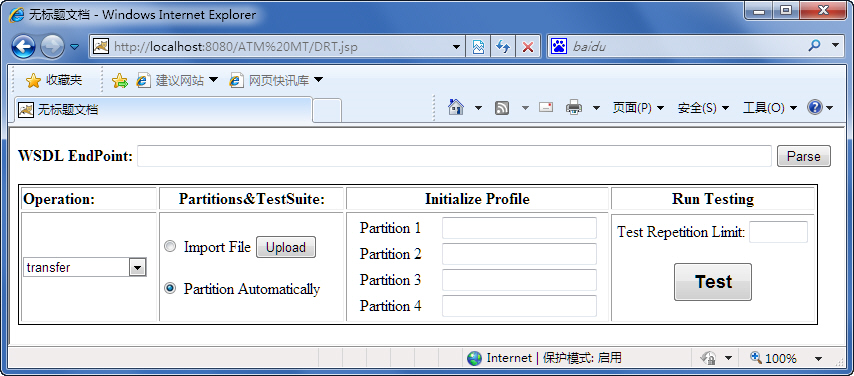
\includegraphics[width=0.5\textwidth]{fig//prototype}
  \caption{Prototype interface}
  \label{fig:prototype}
\end{figure}

\section{Empirical Study}
\label{sec:empiricalstudy}

We conducted a series of empirical studies to evaluate the performance of DRT.

\subsection{Research Questions}
\label{sec:questions}

In our experiments, we focused on addressing the following three research questions:

\begin{description}
  \item [RQ1] How effective is DRT at detecting web service faults?

  Fault-detection effectiveness is a key criterion for evaluating the performance of a testing technique.
  This study used three popular real-life web services as subject programs, and applied mutation analysis to evaluate the effectiveness.

  \item [RQ2] How do the number of partitions and the DRT parameter $\varepsilon$ impact on the failure detection effectiveness and efficiency of DRT?

  In our earlier work~\cite{sun2012towards}, we found that the DRT parameter $\varepsilon$ had a significant effect on DRT efficiency, and  that the optimal value of the parameter could be related to the number of partitions.
  The relationship between $\varepsilon$ and the number of partitions is examined through theoretical analysis, and verified through the empirical studies.

  \item [RQ3] What is the actual test case generation overhead when using the DRT strategy?

  In Section~\ref{sec:DRTStrategy}, we showed that DRT only requires linear time to generate test case.
  We wish to validate the linearity through empirical examination of the actual test case generation and execution.
\end{description}

\subsection{Subject Web Services}
\label{sec:subjects}

We selected three \sout{real-life} web services as the subject programs for our study:
\texttt{Aviation Consignment Management Service (ACMS)},
\texttt{China Unicom billing service (CUBS)}, and
\texttt{Parking billing service (PBS)}, \textcolor{red}{which were developed by ourself based on the real-life specifications.}
We used mutation analysis \cite{demillo1978hints, chen2018test, mao2017out, chen2017similarity} to generate a total of 1563 mutants. Each mutant was created by applying a syntactic change (i.e. mutation operator) to the original program.
We removed equivalent mutants, and mutants that were too easily detected
---
deleting mutants that could be detected with less than 20 randomly generated test cases.
\textcolor{red}{To guarantee the statistic reliability, we first obtained different test suites using 50 random seeds, and tested all mutants on all test suites, then calculated the average number of test cases needed to kill a mutant. Based on the average number, we deleted easily detected mutants.}Table~\ref{tab:objects} summarizes the basic information of the used web services and their mutants.
A detailed description of each web service is given in the following.

\begin{table}
\caption{Studied Web Services}
\label{tab:objects}
\centering
\begin{tabular}{|c|c|c|} \hline
  Web service           &LOC           &Number of mutants \\ \hline
  ACMS    &116           &3   \\ \hline
  CUBS       &131           &11   \\ \hline
  PBS            &129           &4    \\ \hline
\end{tabular}

\end{table}

\subsubsection{Aviation Consignment Management Service (ACMC)}
\label{sec:acms}

ACMS helps airline companies check the allowance (weight) of free baggage, and the cost of additional baggage.
Based on the destination, flights are categorised as either domestic or international.
For international flights, the baggage allowance is greater if the passenger is a student (30kg), otherwise it is 20kg.
Each aircraft offers three cabins classes from which to choose (economy, business, and first), with passengers in different classes having different allowances.
The detailed price rules are summarized in Table~\ref{tab:aviation}, where $price_0$ means economy class fare.

\begin{table*}
  \caption{ACMC Baggage Allowance and Pricing Rules}
  \label{tab:aviation}
  \centering
  \begin{tabular}{|c|c|c|c|c|c|c|} \hline
  \multirow{2}{*}{}     &\multicolumn{3}{c|}{Domestic flights}              &\multicolumn{3}{c|}{International flights} \\
  \cline{2-7}
                       &First class  &Business class   &Economy class   &First class  &Business class   &Economy class \\ \hline
  Carry~on (kg)   &5       &5        &5        &7        &7        &7  \\ \hline
  Free checked-in (kg)   &40      &30       &20       &40       &30       &20/30 \\ \hline
  Additional baggage pricing~(kg)   &\multicolumn{3}{c|}{$price_0 * 1.5\%$}   &\multicolumn{3}{c|}{$price_0 * 1.5\%$}  \\ \hline
  \end{tabular}
\end{table*}

\subsubsection{China Unicom Billing Service (CUBS)}
\label{sec:cubs}

CUBS provides an interface through which customers can know how much they need to pay according to cell-phone plans, calls, and data usage.
The details of several cell-phone plans are summarized in Tables~\ref{table:chinaA},~\ref{table:chinaB}, and~\ref{table:chinaC}.

\begin{table}[h]
  \caption{Plan A}
  \label{table:chinaC}
  \centering
  \begin{tabular}{|c|c|c|c|c|} \hline
  \multicolumn{2}{|c|}{\multirow{2}{*}{Plan details}}  &\multicolumn{3}{|c|}{Month charge~(CNY)} \\ \cline{3-5}
  \multicolumn{2}{|c|}{}                                  &$option_1$  &$option_2$  &$option_3$ \\ \hline
   \multirow{3}{*}{\rotatebox{90}{Basic}} &Free calls~(min)  &260  &380  &550 \\ \cline{2-5}
                                          &Free data~(MB)  &40 &60 &80 \\ \cline{2-5}
                                            &Free data~(MB)  &\multicolumn{3}{c|}{Domestic~(including video calls)} \\ \hline
   \multirow{3}{*}{\rotatebox{90}{Extra}} &Incoming calls~(CNY/min)  &0.25 &0.20  &0.15 \\ \cline{2-5}
                                            &Data~(CNY/KB)  &\multicolumn{3}{c|}{0.0003} \\ \cline{2-5}
                                            &Video calls~(CNY/min)  &\multicolumn{3}{c|}{0.60} \\ \hline
  \end{tabular}
\end{table}

\begin{table*}[hbtp]
  \caption{Plan B}
  \label{table:chinaB}
  \centering
\setlength{\tabcolsep}{1mm}{
  \begin{tabular}{|c|c|c|c|c|c|c|c|} \hline
    \multicolumn{2}{|c|}{\multirow{2}{*}{Plan details}}   &\multicolumn{6}{|c|}{Month charge~(CNY)} \\ \cline{3-8}
    \multicolumn{2}{|c|}{}                                  &\!$option_1$\!  &\!$option_2$\!  &\!$option_3$\!  &\!$option_4$\!  &\!$option_5$\!  \!&$option_6$\!   \\ \hline
    \multirow{3}{*}{\rotatebox{90}{Basic}} &Free calls~(min)  &120  &200  &450  &680  &920  &1180 \\ \cline{2-8}
                                              &Free data~(MB)  &40 &60 &80  &100  &120  &150 \\ \cline{2-8}
                                              &Free incoming calls  &\multicolumn{6}{c|}{Domestic~(including video calls)} \\ \hline
    \multirow{3}{*}{\rotatebox{90}{Extra}} &Incoming calls~(CNY/min)  &0.25 &0.20  &\multicolumn{4}{c|}{0.15} \\ \cline{2-8}
                                              &Data~(CNY/KB)  &\multicolumn{6}{c|}{0.0003} \\ \cline{2-8}
                                              &Video calls~(CNY/min)  &\multicolumn{6}{c|}{0.60} \\ \hline
  \end{tabular}}
\end{table*}

\begin{table*}[hbtp]
  \caption{Plan C}
  \label{table:chinaA}
  \centering
  \resizebox{\textwidth}{12mm}{
  \begin{tabular}{|c|c|c|c|c|c|c|c|c|c|c|c|c|} \hline
  \multicolumn{2}{|c|}{\multirow{2}{*}{Plan details}}                 &\multicolumn{11}{|c|}{Month charge~(CNY)} \\ \cline{3-13}
  \multicolumn{2}{|c|}{}                                                        &\!$option_1$\!  &\!$option_2$\!  &\!$option_3$\!  &\!$option_4$\!  &\!$option_5$\!  &\!$option_6$\! &\!$option_7$\!  &\!$option_8$\!  &\!$option_9$\!  &\!$option_{10}$\!  &\!$option_{11}$\! \\ \hline
  \multirow{3}{*}{\rotatebox{90}{Basic}} &Free calls~(min)  &50  &50  &240  &320  &420  &510  &700 &900 &1250 &1950  &3000 \\ \cline{2-13}
                                            &Free data~(MB)  &150 &300 &300  &400  &500  &650  &750 &950 &1300 &2000  &3000 \\ \cline{2-13}
                                            &Free incoming calls  &\multicolumn{11}{c|}{Domestic~(including video calls)} \\ \hline
  \multirow{3}{*}{\rotatebox{90}{Extra}} &Incoming calls~(CNY/min)  &0.25 &0.20  &\multicolumn{9}{c|}{0.15} \\ \cline{2-13}
                                           &Data~(CNY/KB)  &\multicolumn{11}{c|}{0.0003} \\ \cline{2-13}
                                            &Video calls~(CNY/min)  &\multicolumn{11}{c|}{0.60} \\ \hline
  \end{tabular}}
\end{table*}

\subsubsection{Parking Billing Service (PBS)}
\label{sec:pbs}

Consider a parking billing service that accepts the parking details for a vehicle, including the vehicle type, day of the week, discount coupon, and hours of parking.
This service  rounds up the parking duration to the next full hour, and then calculates the parking fee for according to the hourly rates in Table~\ref{tab:hourlyRate}.
If a discount voucher is presented, a 50\% discount off the parking fee is applied.

\begin{table*}\small
  \caption{Hourly Parking Rates}
  \label{tab:hourlyRate}
  \centering
  \begin{tabular}{|c|c|c|c|c|c|c|} \hline
  \multirow{3}{*}{Actual parking hours}                        &\multicolumn{6}{|c|}{Hourly parking rates} \\ \cline{2-7}
                                   &\multicolumn{3}{|c|}{Weekday}     &\multicolumn{3}{|c|}{Saturday and sunday} \\ \cline{2-7}
                                  &Motorcycle  &Car: 2-door coupe  &Car: others    &Motorcycle  &Car: 2-door coupe  &Car: others \\ \hline
  $(0.0,2.0]$                     &\$4.00        &\$4.50          &\$5.00      &\$5.00        &\$6.00        &\$7.00 \\ \hline
  $(2.0,4.0]$                     &\$5.00        &\$5.50          &\$6.00      &\$6.50      &\$7.50        &\$8.50  \\ \hline
  $(4.0,24.0]$                    &\$6.00        &\$6.50          &\$7.00      &\$8.00      &\$9.00        &\$10.00  \\ \hline
  \end{tabular}
\end{table*}

To facilitate better parking management, at the time of parking, customers may provide an estimation of parking duration, in terms of three different time ranges ($(0.0,2.0]$, $(2.0,4.0]$, and $(4.0,24.0]$).
If the estimation and actual parked hours fall into the same time range, then the customer will receive a 40\% discount;
but if they are different ranges, then a 20\% markup is applied.
A customer may choose to either use a discount coupon, or provide an estimation of parking duration, but may not do both.
No vehicles are allowed to remain parked for two consecutive days on a continuous basis.

\subsection{Variables}
\label{sec:variables}

\subsubsection{Independent Variables}
\label{sec:independentvariables}

The independent variable is the testing technique, DRT.
RPT and RT were used as baseline techniques for comparison.

\subsubsection{Dependent Variables}
\label{sec:dependentvariables}

The dependent variable for RQ1 is the metric for evaluating the fault-detection effectiveness.
Several effectiveness metrics exist, including:
the P-measure~\cite{duran1984evaluation} (the probability of at least one fault being detected by a test suite);
the E-measure~\cite{chen1997optimal} (the expected number of faults detected by a test suite);
the F-measure~\cite{sun2018adaptive} (the expected number of test case executions required to detect the first fault); and
the T-measure~\cite{zhang2014history} (the expected number of test cases required to detect all faults).
Since the F- and T-measures have been widely used for evaluating the fault-detection efficiency and effectiveness of DRT-related testing techniques~\cite{Cai07, cai2009random, Lv2011, Yang2014Dynamic, li2015, zhang2014history}, they are also adopted in this study.
We use $F$ and $T$ to represent the F-measure and the T-measure of a testing method.
As shown in Algorithm~\ref{alg:DRT}, the testing process may not terminate after the detection of the first fault.
Furthermore, because the fault detection information can lead to different probability profile adjustment mechanisms, it is also important to see what would happen after revealing the first fault.
Therefore, we introduce the F2-measure~\cite{sun2018adaptive} as is the number of additional test cases required to reveal the second fault after detection of the first fault.
We use $F2$ to represent the F2-measure of a testing method, and $SD_{measure}$ to represent the standard deviation of metrics (where $measure$ can be $F$, $F2$, or $T$).

An obvious metric for RQ3 is the time required to detect faults.
Corresponding to the T-measure, in this study we used $T$-$time$, the time required to detect all faults.
$F$-$time$ and $F2$-$time$ denote the time required to detect the first fault, and the additional time needed to detect the second fault (after detecting the first), respectively.
For each of these metrics, smaller values indicate a better performance.

\subsection{Experimental Settings}
\label{sec:settings}

\subsubsection{Partitioning}
\label{sec:partition}

In our study, we set the partitions by making use of a decision table (DT) \cite{gettys1986if}.
A DT presents a large amount of complex decisions in a simple, straightforward manner, representing a set of decision rules under all exclusive conditional scenarios in a pre-defined problem.
Typically, a DT consists of four parts:

\begin{enumerate}
	\item
	The upper-left part lists the conditions denoted $C_i$ ($i = 1, \ldots, n$, where $n$ is the number of conditions in the pre-defined problem,
    and $n \ge 1$).
	Each condition $C_i$ contains a set of possible options $O_{i,q} \in CO_i = \{O_{i,1}, \ldots, O_{i,t_{i}}\}$, where $t_i$ is the number of
    possible options for $C_i$, and $q = \{1,\ldots,t_i\}$.
	
	\item
	The upper-right part shows the condition space, which is a Cartesian product of all the $CO_i$	($SP(C) = CO_1 \times CO_2 \times \ldots \times CO_n$).
	Each element in the $SP(C)$ is a condition entry ($CE$) with the ordered $n$-tuple.
	
	\item
	The lower-left part shows all possible actions, represented $A_j$ ($j = 1, \ldots, m$, where $m$ is the number of possible actions and $m \ge 1$).
	Similar to $CO_i$, an action $A_j$ contains a set of possible options $O_{j,p}^{'} \in AO_j = \{O_{j,1}^{'}, \ldots, O_{j,k_{j}}^{'}\}$, where $k_j$ is the number of alternatives for $A_j$, and $p = \{1,\ldots,k_j\}$.

	\item
	The lower-right part shows the action space $SP(A)$, which is also a Cartesian product of all the $AO_j$ ($SP(A) = AO_1 \times AO_2 \times \ldots \times AO_m$).
	Similar to \emph{CE}, each element in the $SP(A)$ is an action entry (\emph{AE}) with the ordered $m$-tuple.
	
\end{enumerate}

A DT \emph{rule} is composed of a \emph{CE} and its corresponding \emph{AE}.
With DT, it is possible to obtain partition schemes with different granularities.
For fine-grain partition schemes, each \emph{CE} of a DT \emph{rule} corresponds to a partition;
while for coarse-grained schemes, a partition corresponds to the union of a group of partitions of which all \emph{CE} of DT \emph{rules} have the same \emph{AE}.
Accordingly, we obtained two partition schemes for each subject web service:
ACMS had 24 and 7 partitions; CUBS, 20 and 3; and PBS, 18 and 3, respectively.

\subsubsection{Initial Test Profile}
\label{sec:profile}

Because test cases may be generated randomly during the test process, a feasible method is to use a uniform probability distribution as the initial testing profile.
On the other hand, testers may also use past experience to guide a different probability distribution as the initial profile.

\subsubsection{Constants}
\label{sec:constant}

In the experiments, we were interested in exploring the relationship between the number of partitions and the DRT strategy parameter $\varepsilon$, and therefore selected a set of parameter values:
$\varepsilon \in \{1.0E$-$05, 5.0E$-$05, 1.0E$-$04, 5.0E$-$04, 1.0E$-$03, 5.0E$-$03, 1.0E$-$02, 5.0E$-$02, 1.0E$-$01, 2E$-$01, 3E$-$01, 4E$-$01, 5E$-$01\}$.
It should be noted that $\varepsilon = 5E$-$01$ is already a large value.
Consider the following scenario.
For PBS, when the test is carried out under partition scheme 2, if $\varepsilon = 7.5E$-$01$ and  a uniform probability distribution is used as the testing profile (that is, $p_i = 1/3$) , then suppose that the first test case belonging to $c_1$ is executed and does not reveal any faults, then, according to Formula 3, the value of $p_1$ would become $0$.
It is important, therefore, that the initial value of $\varepsilon$ should not be set too large.

\subsection{Experimental Environment}
\label{sec:environment}

Our experiments were conducted on a virtual machine running the Ubuntu 11.06 64-bit operating system, with two CPUs, and a memory of 2GB.
The test scripts were written in Java.
To ensure statistically reliable values \cite{arcuri2011practical} of the metrics (F-measure, F2-measure, T-measure, F-time, F2-time, and T-time), each testing session was repeated 30 times with 30 different seeds, and the average value calculated.

\subsection{Threats To Validity}
\label{sec:threats}

\subsubsection{Internal Validity}
\label{sec:internalthreats}

A threat to internal validity is related to the implementations of the testing techniques, which involved a moderate amount of programming work.
However, our code was cross-checked by different individuals, and we are confident that all techniques were correctly implemented.

\subsubsection{External Validity}
\label{sec:externalthreats}

The possible threat to external validity is related to the subject programs and seeded faults under evaluation.
Although the three subject web services are not very complex, they do implement real-life business scenarios of diverse application domains.
Furthermore, 18 distinct faults were used to evaluate the performance.
These faults cover different types of mutation operators and require an average of more than 20 randomly generated test cases to be detected.
Although we have tried to improve the generalisability of the findings by applying different partitioning granularities, and 13 kinds of parameters, we cannot be certain that similar results would be observed in other types of web services.

\subsubsection{Construct Validity}
\label{sec:construct}

The metrics used in our study are simple in concept and straightforward to apply, and hence there should be little threat to the construct validity.

\subsubsection{Conclusion Validity}
\label{sec:conclusion}

As reported for empirical studies in the field of software engineering \cite{arcuri2011practical},  at least 30 observations are necessary to ensure the statistical significance of results.
Accordingly, we have run a sufficient number of trials to ensure the  reliability of our experimental results.
Furthermore, as will be discussed in Section~\ref{sec:results}, further statistical tests were also conducted to confirm their significance.

\section{Experimental Results}
\label{sec:results}

\subsection{RQ1: Fault Detection Effectiveness}
\label{sec:RQ1}

The distributions of F-, F2-, and T-measure results for each program are displayed using boxplots in
Figures~\ref{fig:Fmeasure} to~\ref{fig:Tmeasure}.
In each boxplot, the upper and lower bounds of the box represent the third and first quartiles of the metric, respectively;
the middle line represents the median value;
the upper and lower whiskers mark, respectively, the largest and smallest data within the range of $\pm 1.5 \times IQR$ (where $IQR$ is the interquartile range);
outliers beyond the  $IQR$ are denoted with hollow circles; and
each solid circle represents the mean value of the metric.
\begin{figure*}
	\centering
    \subfigure[ACMS] {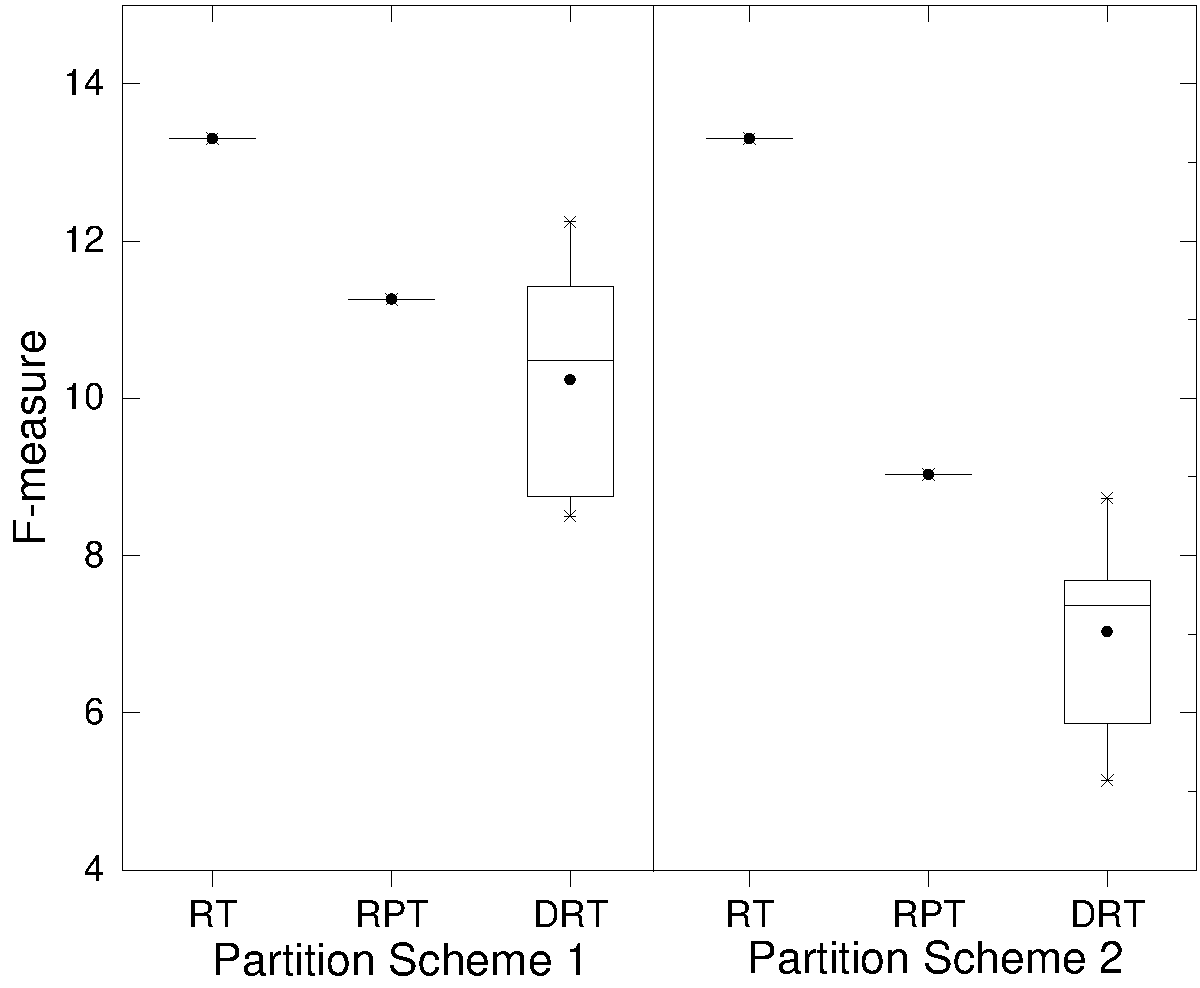
\includegraphics[width=0.32\textwidth,height=4cm]{fig/drtresultbox/aviaresultf.pdf}}
	\subfigure[CUBS] {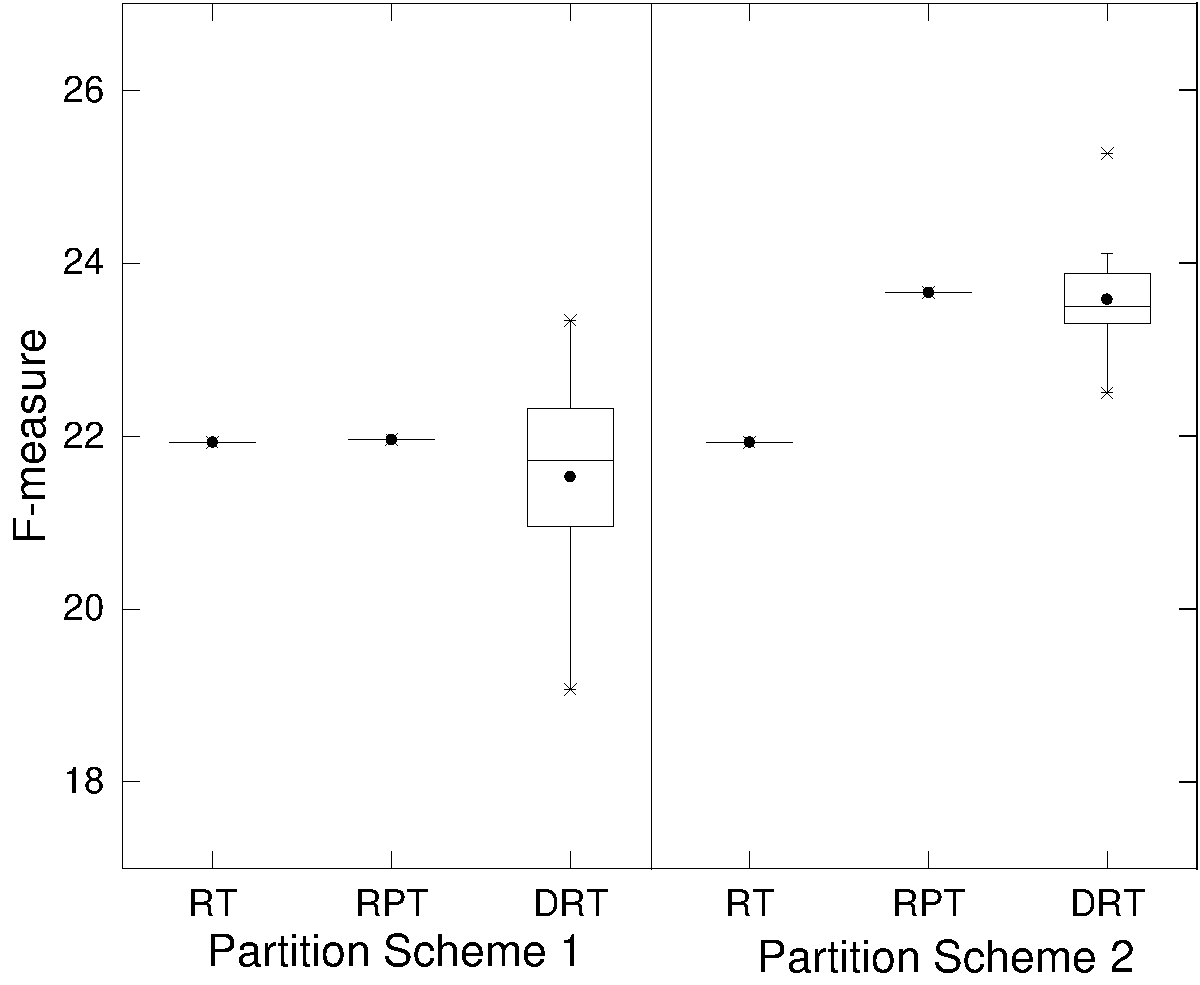
\includegraphics[width=0.32\textwidth,height=4cm]{fig/drtresultbox/chinaresultf.pdf}}
	\subfigure[PBS] {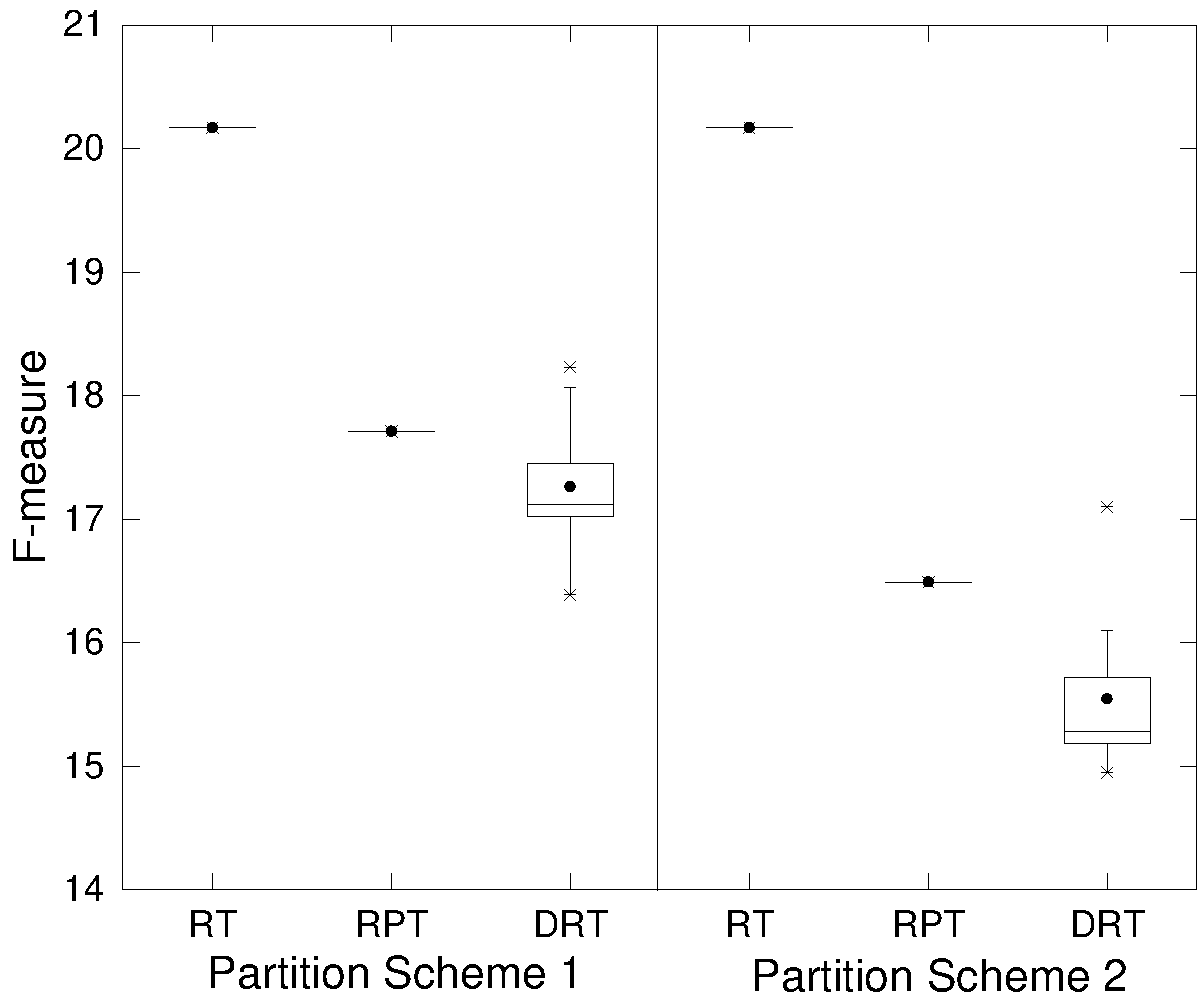
\includegraphics[width=0.32\textwidth,height=4cm]{fig/drtresultbox/parkingresultf.pdf}}
	\caption{F-measure boxplots for each program}
	\label{fig:Fmeasure}
\end{figure*}

\begin{figure*}
	\centering
	\subfigure[ACMS] {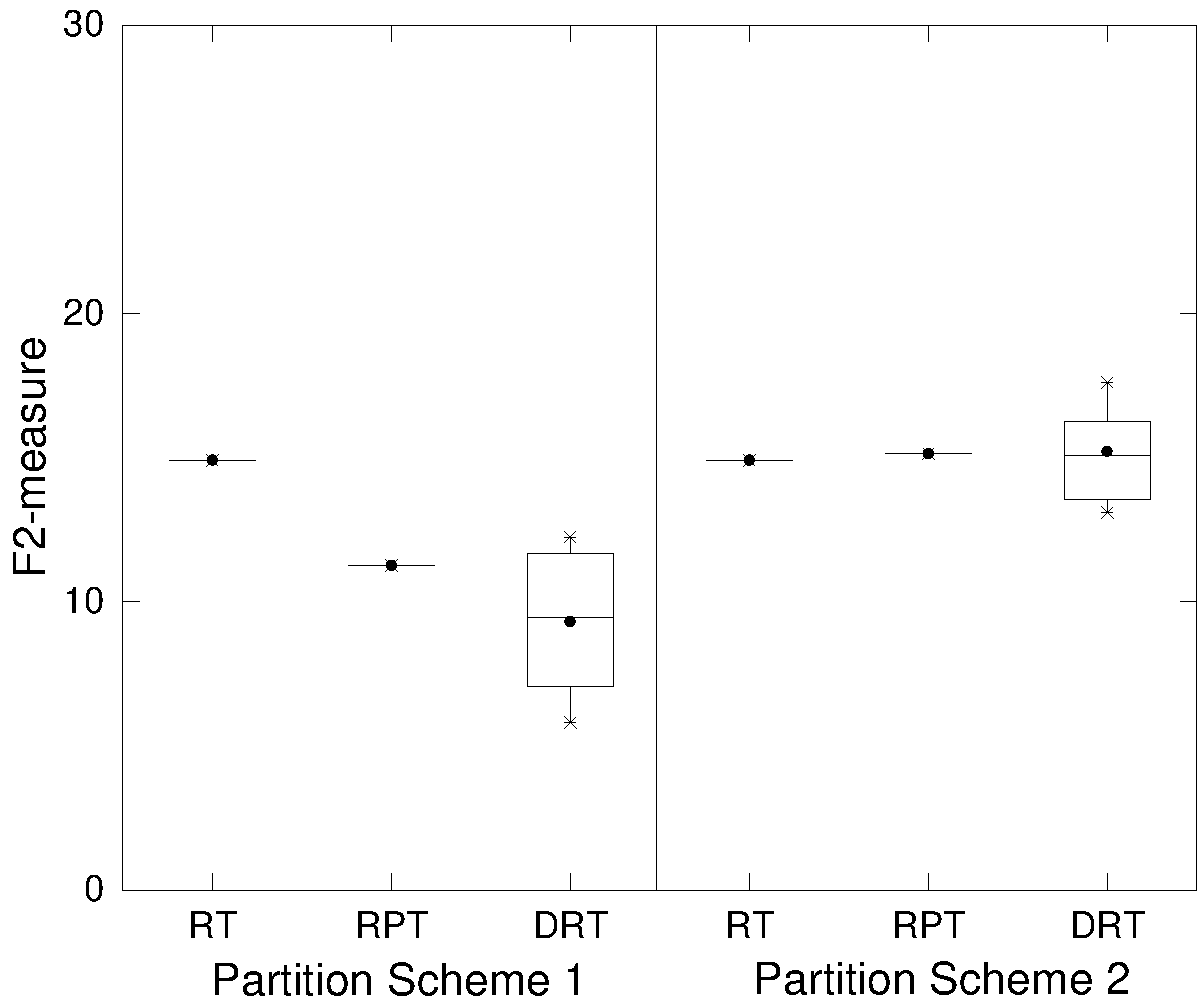
\includegraphics[width=0.32\textwidth,height=4cm]{fig/drtresultbox/aviaresultf2.pdf}}
	\subfigure[CUBS] {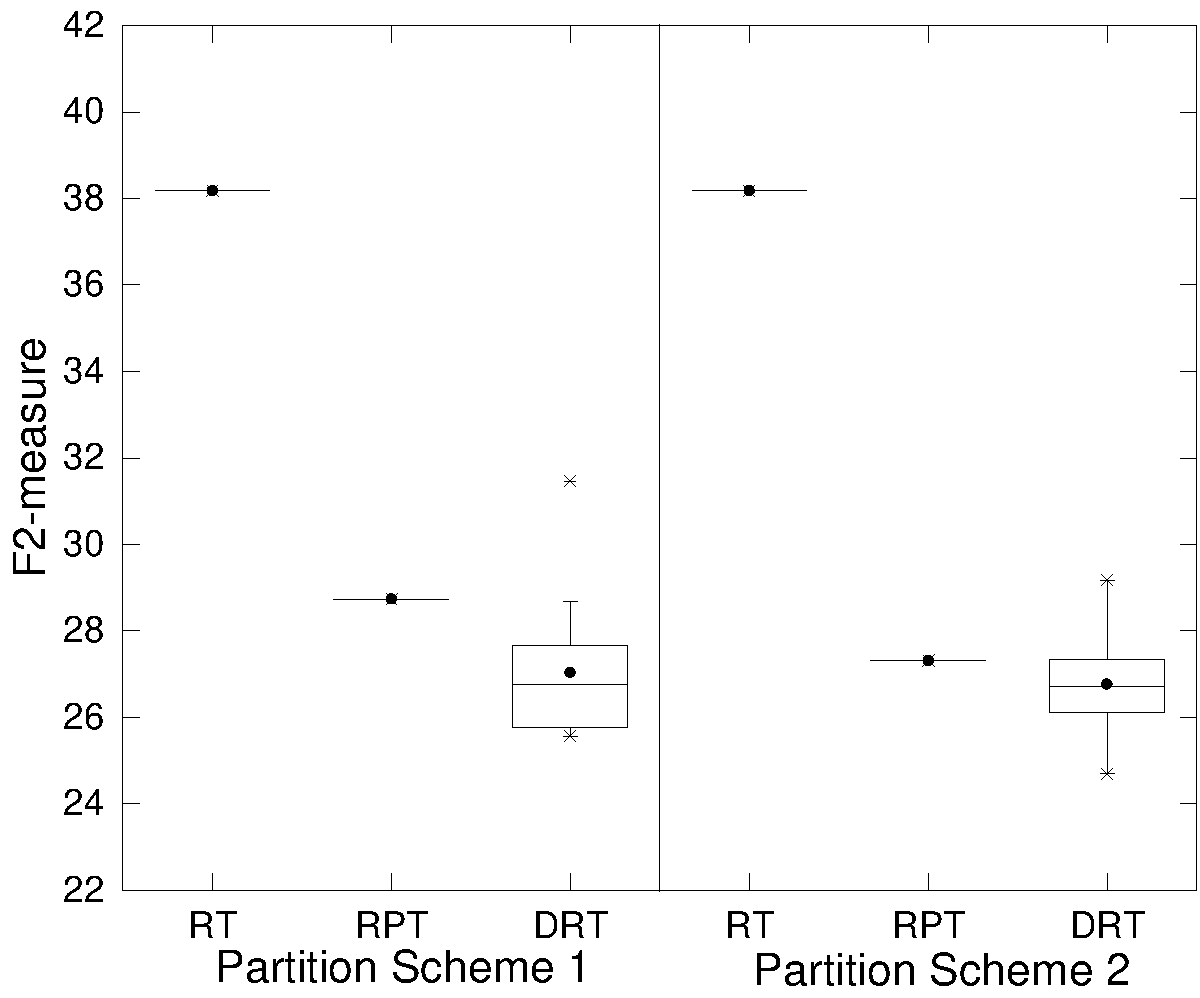
\includegraphics[width=0.32\textwidth,height=4cm]{fig/drtresultbox/chinaresultf2.pdf}}
	\subfigure[PBS] {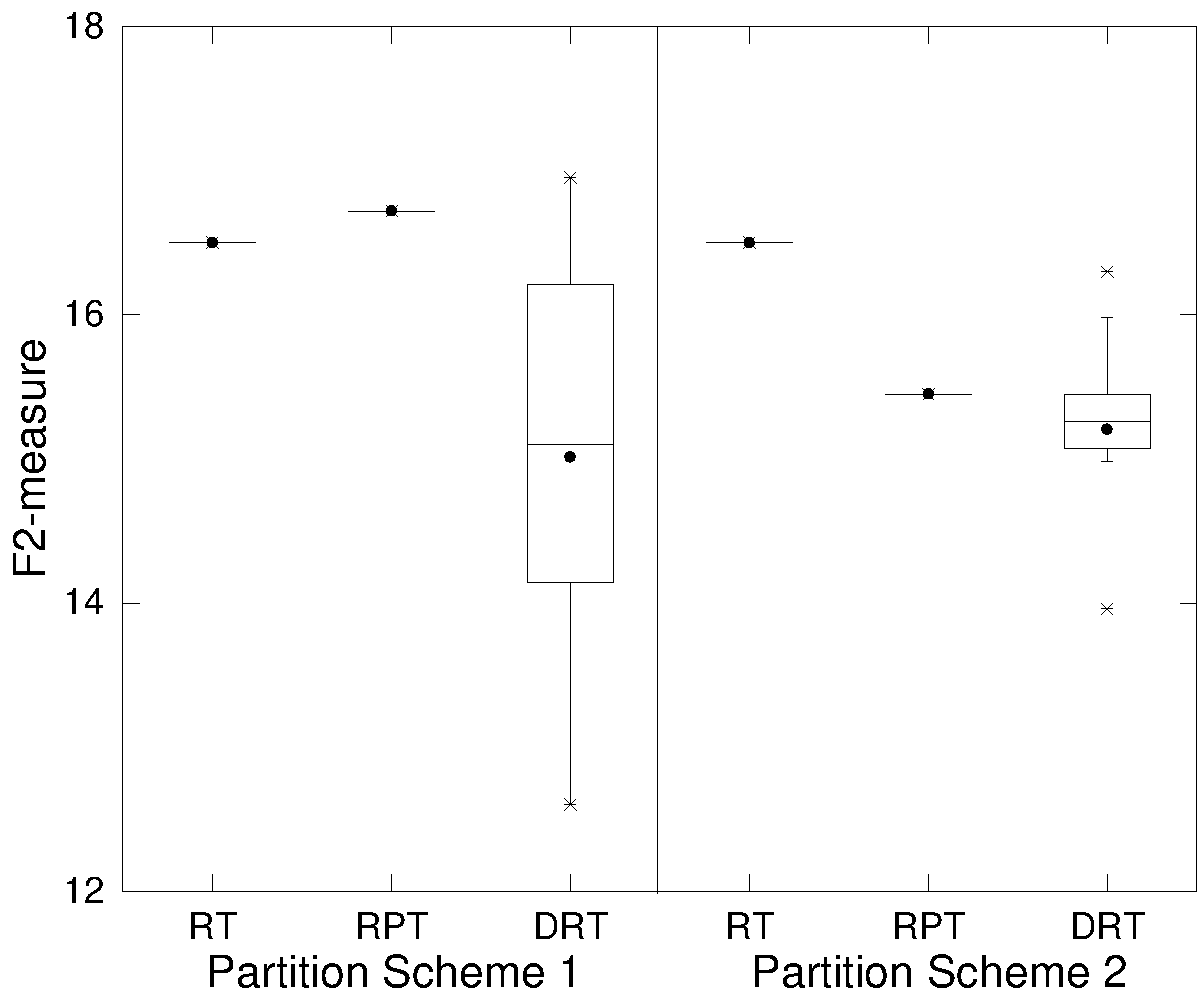
\includegraphics[width=0.32\textwidth,height=4cm]{fig/drtresultbox/parkingresultf2.pdf}}
	\caption{F2-measure boxplots for each program}
	\label{fig:F2measure}
\end{figure*}

\begin{figure*}
	\centering
	\subfigure[ACMS] {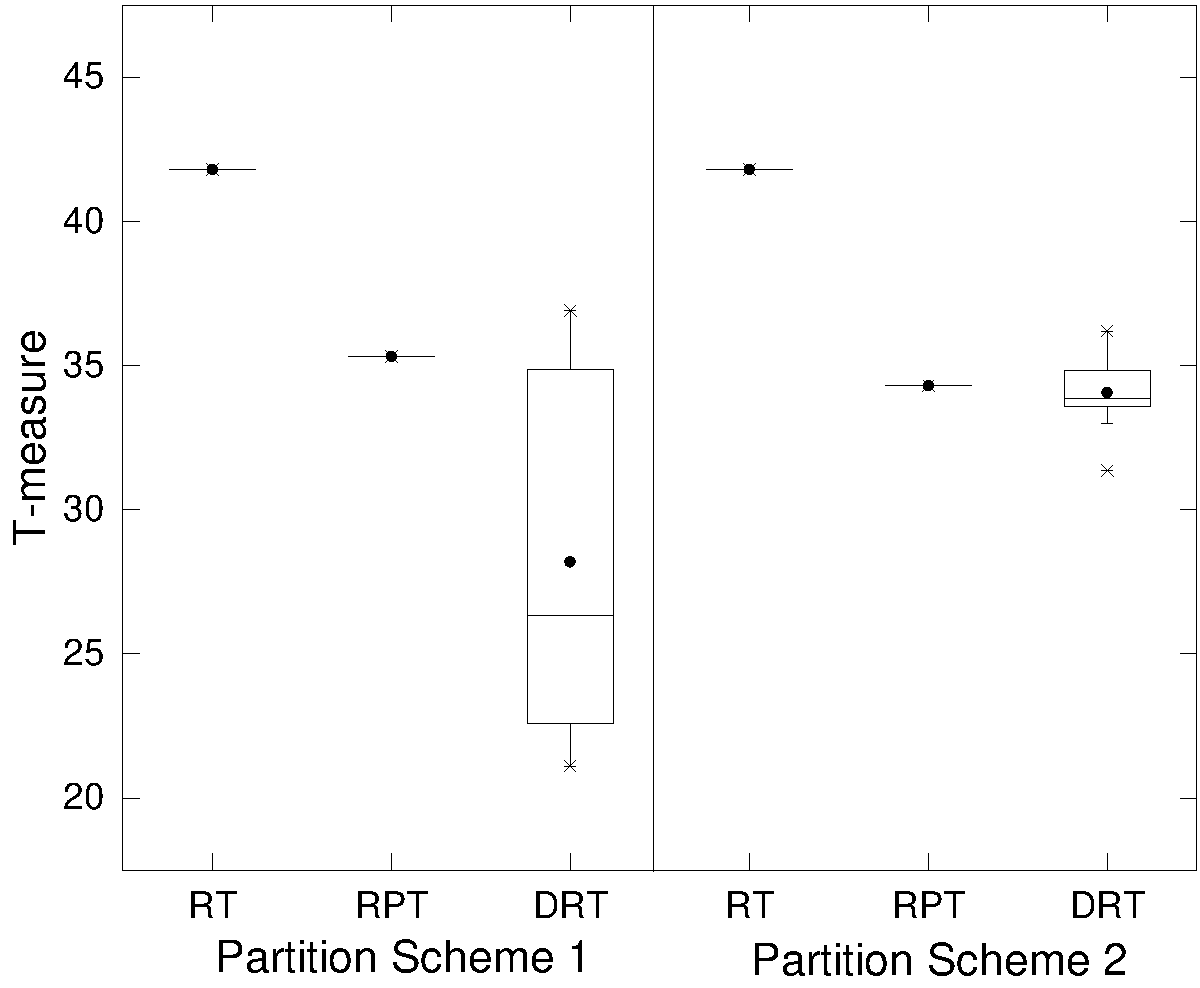
\includegraphics[width=0.32\textwidth,height=4cm]{fig/drtresultbox/aviaresultt.pdf}}
	\subfigure[CUBS] {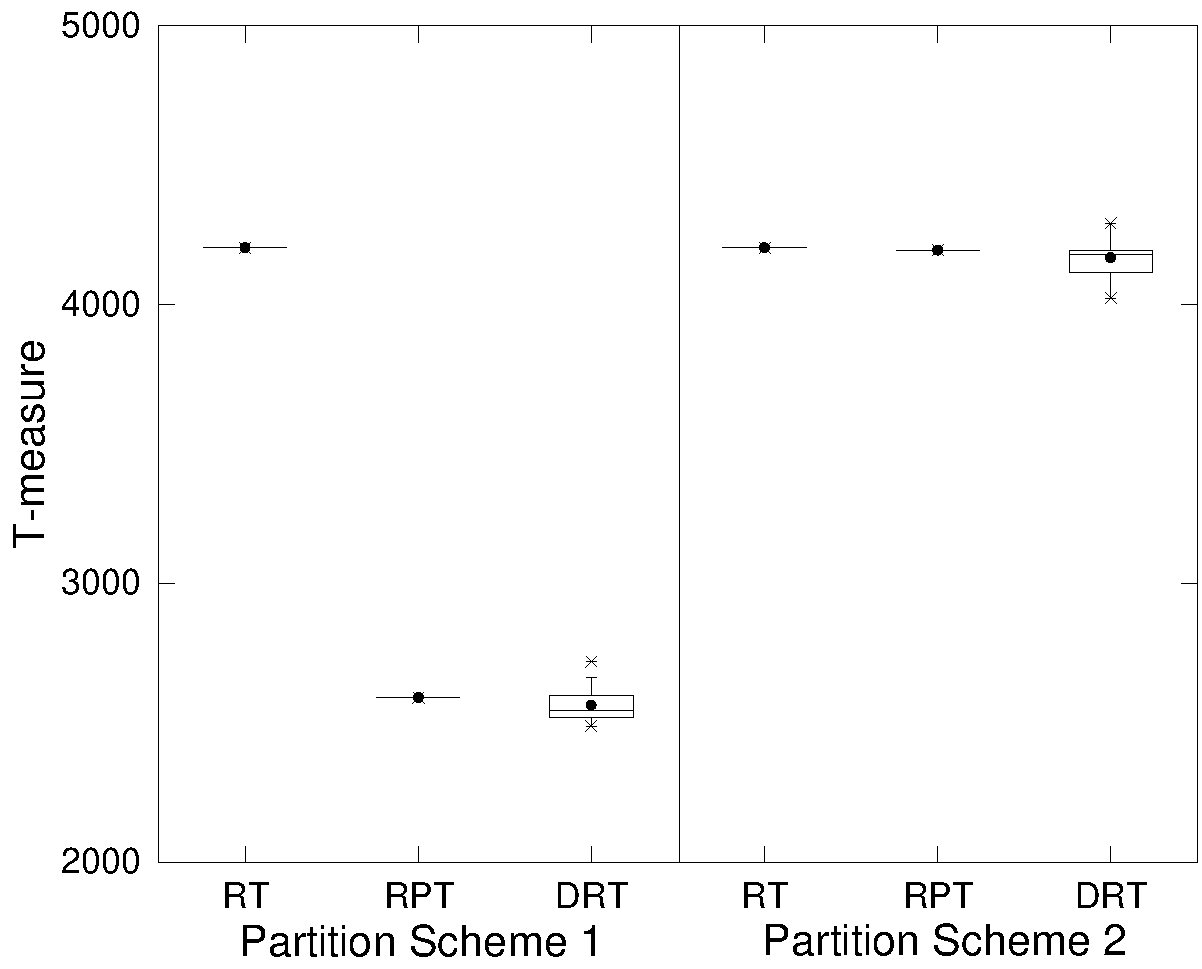
\includegraphics[width=0.32\textwidth,height=4cm]{fig/drtresultbox/chinaresultt.pdf}}
	\subfigure[PBS] {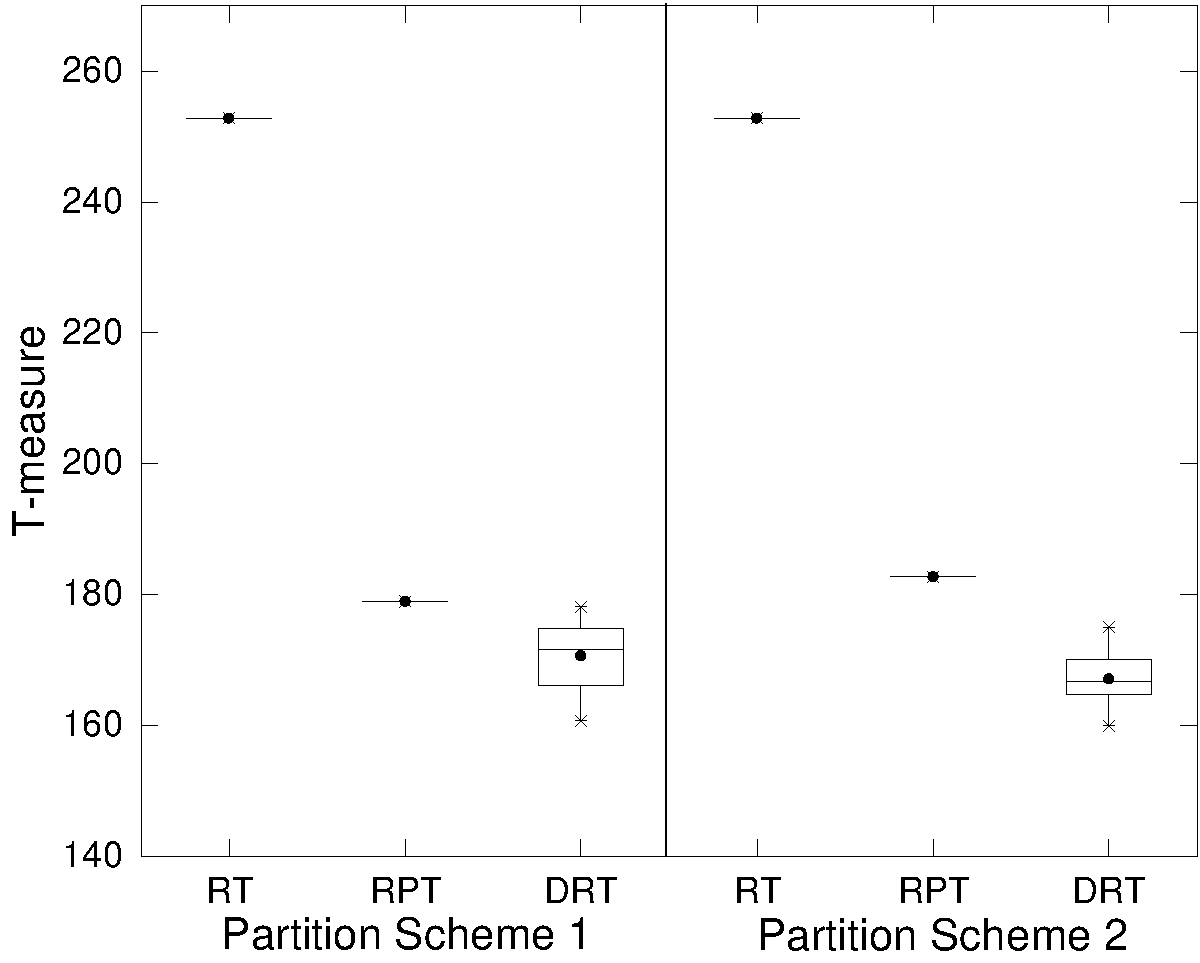
\includegraphics[width=0.32\textwidth,height=4cm]{fig/drtresultbox/parkingresultt.pdf}}
	\caption{T-measure boxplots for each program}
	\label{fig:Tmeasure}
\end{figure*}

It can observed from the tables and figures that, in general, DRT is the best performer, followed by RPT.
We also conducted statistical testing to verify the significance of this observation, using the Holm-Bonferroni method~\cite{sun2018adaptive} (with p-value equal to $0.05$) to determine which pairs of testing techniques had significant differences.
The statistical data are shown in Table \ref{tableHlom:f/f2/t-measure}, where each cell gives the number of scenarios where the technique above (in the table) performed better than one to the left.
Where the difference is significant, the number is underlined and in bold face.
For example, the \underline{\textbf{75}} in the top right cell of Table~\ref{tableHlom:f/f2/t-measure} indicates that, of 78 scenarios (13 parameters $\times$ two partition schemes $\times$ three web services), DRT had lower F2-measure scores than RT for 75, with the fault-detection capabilities of these two techniques being significantly different.

\begin{table}[htbp]
  \caption{Number of Scenarios Where the Technique on the Top Wow Has a Lower Metric (F-/F2/T-measure) Score Than That on The Left Column}
  \centering
  \label{tableHlom:f/f2/t-measure}
  \begin{tabular}{|c|c|c|c|c|c|c|c|c|c|}  \hline
  \multirow{2}{*}{}  &\multicolumn{3}{|c|}{F-measure}                  &\multicolumn{3}{|c|}{F2-measure}        &\multicolumn{3}{|c|}{T-measure} \\ \cline{2-10}
                     & \!RT\!    &  \!RPT\!    &\!DRT\!                & \!RT\!    &  \!RPT\!    &\!DRT\!       & \!RT\!    &  \!RPT\!    &\!DRT\!           \\ \hline
  RT                 & ---   &4        &\underline{\textbf{60}}        & ---   &4     &\underline{\textbf{69}}  & ---   &6   &\underline{\textbf{75}}  \\ \hline
  RPT                &2      & ---     &\underline{\textbf{62}}        &2      & ---  &\underline{\textbf{63}}  &0      &---     &\underline{\textbf{64}} \\ \hline
  DRT&\underline{\textbf{18}}&\underline{\textbf{16}}&---&\underline{\textbf{9}} &\underline{\textbf{15}} &--- &\underline{\textbf{3}}  &\underline{\textbf{14}} & ---  \\ \hline
  \end{tabular}
\end{table}


Table~\ref{tableHlom:f/f2/t-measure} clearly shows that the difference between each pair of testing techniques is always significantly different.

\subsection{RQ2: Relationship between Partition Number and $\varepsilon$}
\label{sec:RQ2}

In~\ref{sec:relation}, we analyzed the relationship between the number of partitions and the DRT strategy parameter $\varepsilon$.
In this section, we show that our theoretical analysis provides useful guidance to testers to set the value of $\varepsilon$.

We used three web services to validate our theoretical analysis.
Before starting the test, the failure rate $\theta_i$ of partition $s_i$ was obtained by executing ($k$) test cases from $s_i$ until revealing a fault, then $\theta_i = k / k_i$, where $k_i$ is the total number of test cases in $s_i$.
According to Formula 19, the theoretically optimal values of~$\varepsilon$ in each scenario for each web service are shown in Table~\ref{tab:parameters}, where $\varepsilon^{*}$ denotes the theoretical value of $\varepsilon$.
We ran a series of experiments with the parameters set according to those in Table~\ref{tab:parameters}\sout{:
The F-, F2-, and T-measure results for each  program are shown in Figure~\ref{fig:theovsnontheo},}.
\textcolor{red}{Figure \ref{fig:theovsnontheo} shows, for each scenario, how many times DRT with theoretical parameter required less than test cases than DRT with normal parameters described in Section \ref{sec:constant} -- i.e., DRT with theoretical parameter ``wins'' the comparison; how many times DRT normal parameters required less test cases (normal values win). Apart from the DRT strategy parameter $\varepsilon$, all other experimental settings remained the same as in Section~\ref{sec:RQ1}.}
%
%\textcolor{red}{where we used $log_{100}(1.0E05 \times \varepsilon)$ for the horizontal axis to ease of presentation and understanding. The additional elements $\varepsilon_1^{*}$ and $\varepsilon_2^{*}$ denote the values of $log_{100}(1.0E05 \times \varepsilon^{*})$ in different partition scheme for each studied web service. Apart from the DRT strategy parameter $\varepsilon$, all other experimental settings remained the same as in Section~\ref{sec:RQ1}.}
\begin{figure}[h]
	\centering
    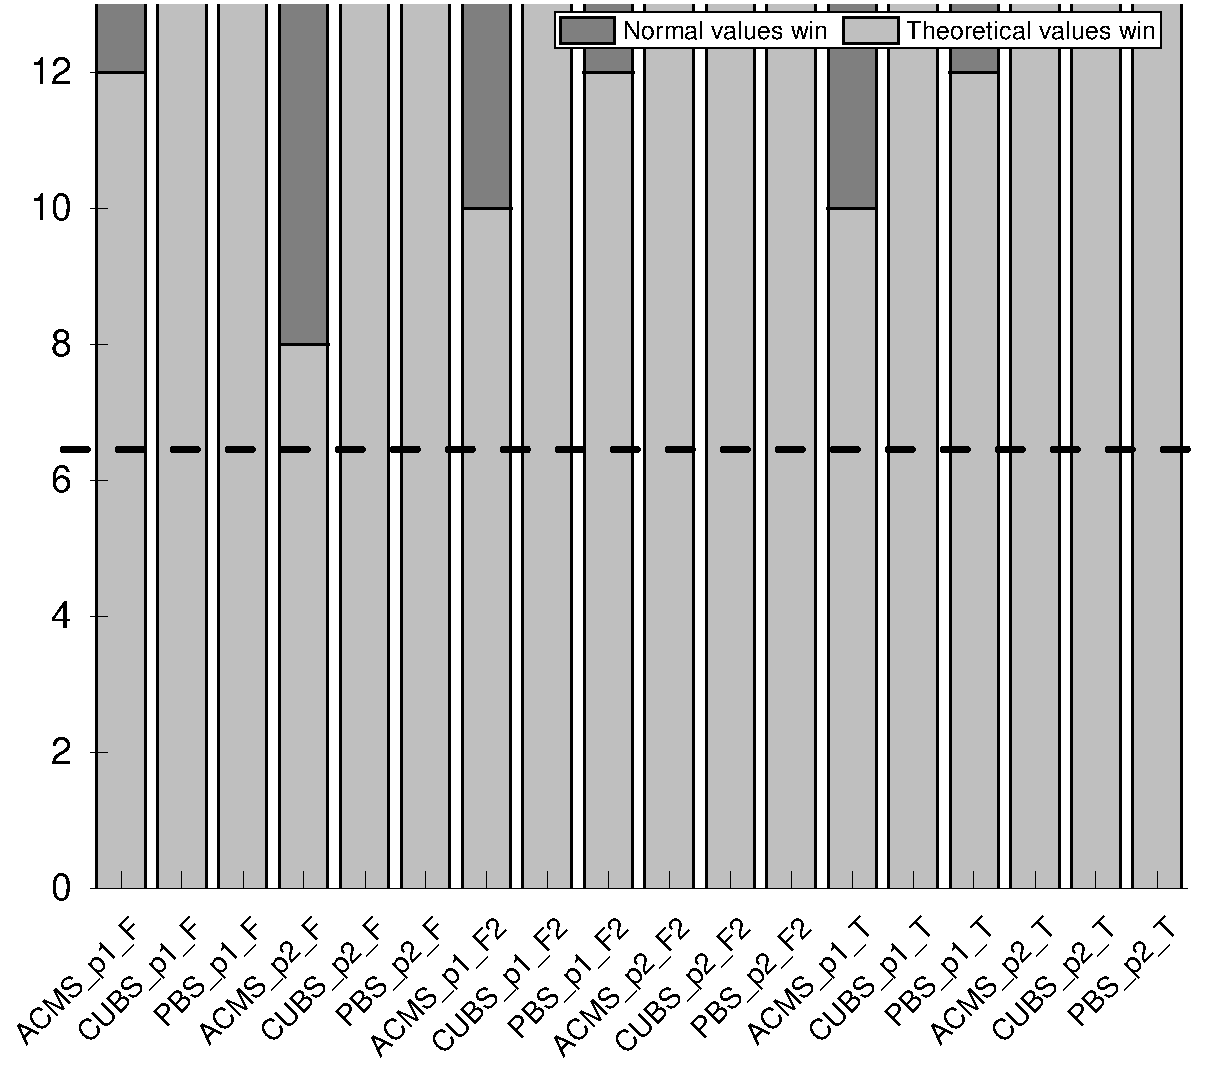
\includegraphics[width=0.5\textwidth]{fig/drtparemeter/theVSnor.pdf}
	\caption{Test Selection: number of wins of DRT with theoretical parameters and DRT with normal parameters}
	\label{fig:theovsnontheo}
\end{figure}

%$\varepsilon_1^{*}$ and $\varepsilon_2^{*}$ denote the theoretical values of parameter $\varepsilon$ in the two different partition schemes, respectively.For ease of presentation and understanding, we used $log_{100}(1.0E05 \times \varepsilon)$ for the horizontal axis in Figure \ref{fig:theovsnontheo}. Apart from the DRT strategy parameter $\varepsilon$, all other experimental settings remained the same as in Section~\ref{sec:RQ1}}.

\begin{table}
  \caption{Theoretical Optimal Values of DRT Parameter}
  \centering
  \label{tab:parameters}
  \begin{tabular}{|c|c|c|c|} \hline
     Web                         & Partition  &$\theta_{min}$   &$\varepsilon^{*}$             \\
     service                   & scheme     &                 &                \\ \hline
     \multirow{2}{*}{ACMS}       &1           &5.452E-2         &1.601E-1        \\ \cline{2-4}
                                 &2           &2.797E-3         &1.102E-4        \\ \hline
     \multirow{2}{*}{CUBS}       &1           &1.193E-3         &5.702E-5        \\ \cline{2-4}
                                 &2           &1.397E-3         &1.734E-5        \\ \hline
     \multirow{2}{*}{PBS}        &1           &1.760E-3         &1.118E-4        \\ \cline{2-4}
                                 &2           &1.492E-3         &1.340E-5        \\ \hline
  \end{tabular}
\end{table}

From Figure~\ref{fig:theovsnontheo}, we have the following observations:
\begin{itemize}
  \item
  In most scenarios, the DRT strategy with theoretically optimum parameter value performs best.
  Furthermore, the DRT strategy performs better when the parameter values are near the theoretically optimum value than when not.

  \item
  From Figure \ref{fig:theovsnontheo} (a), it can be observed that the DRT strategy with larger parameter values performs better than with the theoretically optimum value, in terms of the F-measure.
  The main reason for this is that, for this scenario, the maximum failure rate ($\theta_M = 4.781E-3$) is large and the number of partitions is small:
  When the parameter value is large, the probability of selecting partitions with lower failure rates is quickly reduced, and the probability of selecting partitions with larger failure rates is quickly increased, according to Formulas 3 and 4.

\end{itemize}

\subsection{RQ3: Selection Overhead}
\label{sec:RQ3}

Tables~\ref{tab:timeavia} to~\ref{tab:timeparking} summarize the F-, F2-, and T-time results, respectively, and their distributions for each web service is shown in Figures~\ref{fig:Ftime} to \ref{fig:Ttime}.
It can be observed from the figures that, in general, DRT had the best performance, and RPT just marginally outperforms RT.

\begin{table}[hbt]
  \caption{F-time, F2-time and T-time for Web Service ACMS (in ms)}
  \label{tab:timeavia}
  \centering
  \setlength{\tabcolsep}{1mm}{
  \begin{tabular}{|c|c|c|c|c|c|c|c|} \hline
     \multicolumn{2}{|c|}{\multirow{2}{*}{Strategy}} &\multicolumn{3}{|c|}{Partition scheme 1} &\multicolumn{3}{|c|}{Partition scheme 2}\\ \cline{3-8}
     \multicolumn{2}{|c|}{}    &F-time	&F2-time &T-time &F-time &F2-time &T-time  \\ \hline
     \multicolumn{2}{|c|}{RT}  &0.43	&0.29	&0.85	&0.43 	&0.29	&0.85   \\ \hline
     \multicolumn{2}{|c|}{RPT} &0.57	&0.31	&1.08	&0.33	&0.45	&0.78   \\ \hline
         \multirow{13}{*}{DRT} &1.0E-5    &0.47	&0.28	&0.96	&0.38	&0.41	&0.95  \\ \cline{2-8}
                               &5.0E-5	  &0.35	&0.21	&0.78	&0.30	&0.27	&0.71 \\ \cline{2-8}
                               &1.0E-4	  &0.33	&0.19	&0.66	&0.24	&0.28	&0.65 \\ \cline{2-8}
                               &5.0E-4	  &0.30	&0.17	&0.60	&0.27	&0.25	&0.67 \\ \cline{2-8}
                               &1.0E-3	  &0.29	&0.19	&0.61	&0.22	&0.24	&0.60 \\ \cline{2-8}
                               &5.0E-3	  &0.28	&0.23	&0.62	&0.21	&0.31	&0.64 \\ \cline{2-8}
                               &1.0E-2	  &0.24	&0.17	&0.53	&0.23	&0.29	&0.66 \\ \cline{2-8}
                               &5.0E-2	  &0.28	&0.13	&0.49	&0.23	&0.35	&0.71 \\ \cline{2-8}
                               &1.0E-1	  &0.26	&0.08	&0.43	&0.23	&0.29	&0.63 \\ \cline{2-8}
                               &2.0E-1	  &0.23	&0.12	&0.43	&0.30	&0.46	&0.89 \\ \cline{2-8}
                               &3.0E-1	  &0.24	&0.11	&0.45	&0.18	&0.40	&0.69 \\ \cline{2-8}
                               &4.0E-1	  &0.27	&0.10	&0.47	&0.16	&0.31	&0.58 \\ \cline{2-8}
                               &5.0E-1	  &0.28	&0.11	&0.47	&0.28	&0.45	&0.86 \\ \hline
  \end{tabular}}
\end{table}


\begin{table}[hbt]
  \caption{F-time, F2-time and T-time for Web Service CUBS (in ms)}
  \label{tab:timechina}
  \centering
  \setlength{\tabcolsep}{1mm}{
  \begin{tabular}{|c|c|c|c|c|c|c|c|} \hline
     \multicolumn{2}{|c|}{\multirow{2}{*}{Strategy}} &\multicolumn{3}{|c|}{Partition scheme 1} &\multicolumn{3}{|c|}{Partition scheme 2}\\ \cline{3-8}
     \multicolumn{2}{|c|}{}    &F-time	&F2-time &T-time &F-time &F2-time &T-time  \\ \hline
     \multicolumn{2}{|c|}{RT}  &0.82	&1.14	&34.69	&0.82	&1.14	&34.69   \\ \hline
     \multicolumn{2}{|c|}{RPT} &0.91	&0.87	&30.54	&0.75	&0.79	&34.59   \\ \hline
         \multirow{13}{*}{DRT} &1.0E-5    &0.91	&0.87	&30.14	&0.87	&0.83	&36.49  \\ \cline{2-8}
                               &5.0E-5	  &0.95	&0.86	&30.21	&0.82	&0.75	&34.70\\ \cline{2-8}
                               &1.0E-4	  &0.77	&0.89	&29.27	&0.86	&0.69	&35.34 \\ \cline{2-8}
                               &5.0E-4	  &0.79	&1.00	&31.05	&0.87	&0.90	&36.85 \\ \cline{2-8}
                               &1.0E-3	  &0.86	&0.88	&29.93	&0.92	&0.77	&36.44 \\ \cline{2-8}
                               &5.0E-3	  &0.86	&0.83	&30.28	&0.83	&0.83	&36.27 \\ \cline{2-8}
                               &1.0E-2	  &0.95	&0.88	&29.33	&0.84	&0.72	&35.23 \\ \cline{2-8}
                               &5.0E-2	  &0.84	&0.82	&30.56	&0.88	&0.72	&37.07 \\ \cline{2-8}
                               &1.0E-1	  &0.88	&0.93	&29.45	&0.82	&0.76	&37.14 \\ \cline{2-8}
                               &2.0E-1	  &0.83	&0.83	&30.16	&0.86	&0.73	&36.79 \\ \cline{2-8}
                               &3.0E-1	  &0.95	&0.86	&27.81	&0.84	&0.84	&36.89 \\ \cline{2-8}
                               &4.0E-1	  &0.84	&0.84	&28.23	&0.86	&0.82	&35.22 \\ \cline{2-8}
                               &5.0E-1	  &0.87	&0.84	&27.91	&0.90	&0.86	&38.21 \\ \hline
  \end{tabular}}
\end{table}

\begin{table}[hbt]
  \caption{F-time, F2-time and T-time for Web Service PBS (in ms)}
  \label{tab:timeparking}
  \centering
  \setlength{\tabcolsep}{1mm}{
  \begin{tabular}{|c|c|c|c|c|c|c|c|} \hline
     \multicolumn{2}{|c|}{\multirow{2}{*}{Strategy}} &\multicolumn{3}{|c|}{Partition scheme 1} &\multicolumn{3}{|c|}{Partition scheme 2}\\ \cline{3-8}
     \multicolumn{2}{|c|}{}    &F-time	&F2-time &T-time &F-time &F2-time &T-time  \\ \hline
     \multicolumn{2}{|c|}{RT}  &0.81	&0.42	&4.12	&0.81	&0.42	&4.12   \\ \hline
     \multicolumn{2}{|c|}{RPT} &0.85	&0.52	&3.83	&0.66	&0.35	&2.98   \\ \hline
         \multirow{13}{*}{DRT} &1.0E-5    &0.76	&0.48	&3.85	&1.05	&0.51	&3.44  \\ \cline{2-8}
                               &5.0E-5    &0.73	&0.35	&3.02	&0.91	&0.52	&3.79\\ \cline{2-8}
                               &1.0E-4    &0.54	&0.36	&2.97	&0.49	&0.34	&2.26 \\ \cline{2-8}
                               &5.0E-4    &0.68	&0.34	&3.20	&0.50	&0.30	&2.31 \\ \cline{2-8}
                               &1.0E-3    &0.62	&0.38	&2.87	&0.52	&0.38	&2.42 \\ \cline{2-8}
                               &5.0E-3    &0.60	&0.38	&2.99	&0.43	&0.51	&2.40 \\ \cline{2-8}
                               &1.0E-2    &0.58	&0.42	&2.84	&0.51	&0.34	&2.41 \\ \cline{2-8}
                               &5.0E-2    &0.64	&0.44	&3.27	&0.59	&0.36	&2.49 \\ \cline{2-8}
                               &1.0E-1    &0.65	&0.38	&3.46	&0.60	&0.38	&2.56 \\ \cline{2-8}
                               &2.0E-1	  &0.60	&0.36	&3.22	&0.54	&0.59	&2.47 \\ \cline{2-8}
                               &3.0E-1	  &0.59	&0.44	&3.24	&0.57	&0.46	&2.57 \\ \cline{2-8}
                               &4.0E-1	  &0.61	&0.33	&2.90	&0.51	&0.33	&2.54 \\ \cline{2-8}
                               &5.0E-1	  &0.62	&0.44	&3.16	&0.56	&0.36	&2.56 \\ \hline
  \end{tabular}}
\end{table}

\begin{figure*}
	\centering
    \subfigure[ACMS] {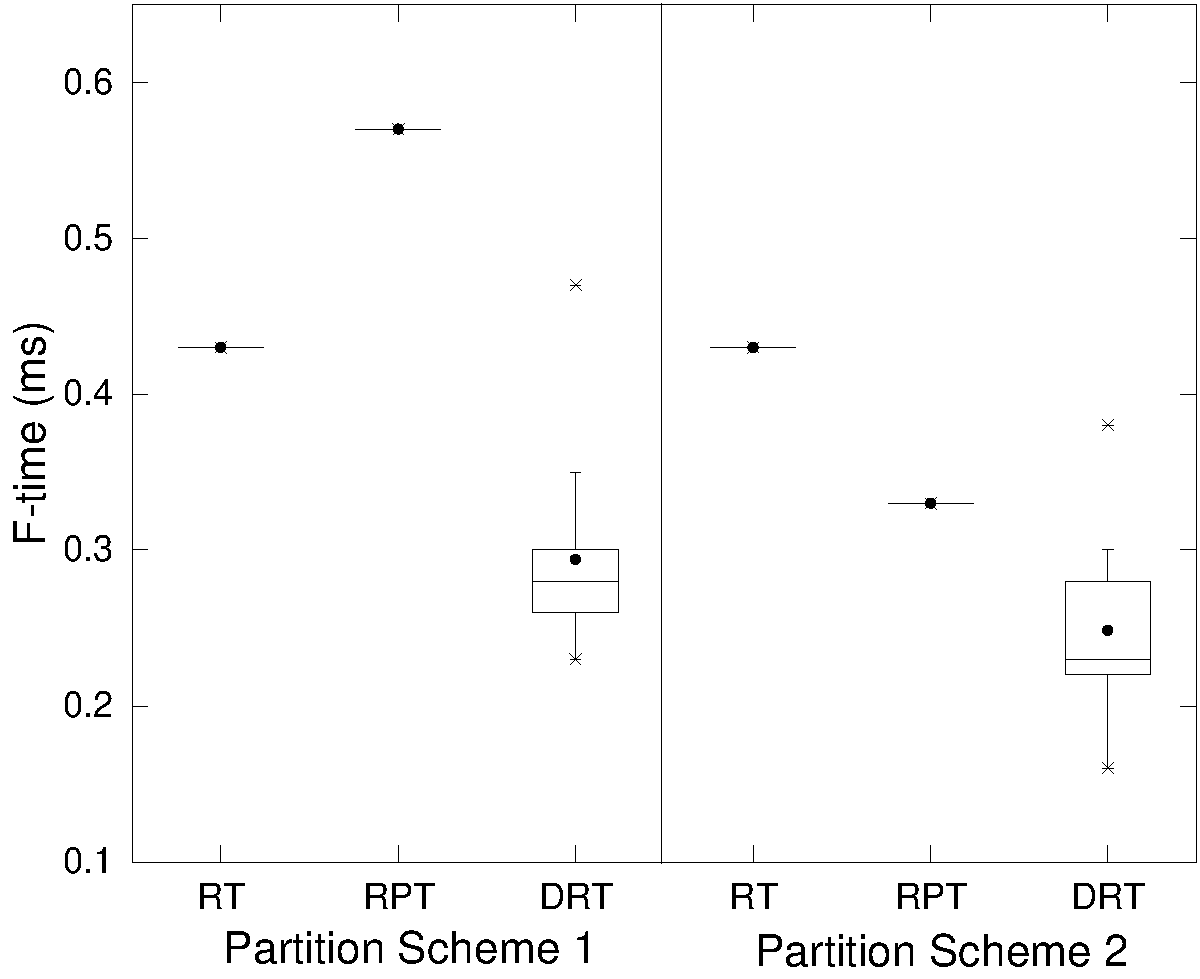
\includegraphics[width=0.32\textwidth,height=4cm]{fig/drttime/aviatimef}}
	\subfigure[CUBS] {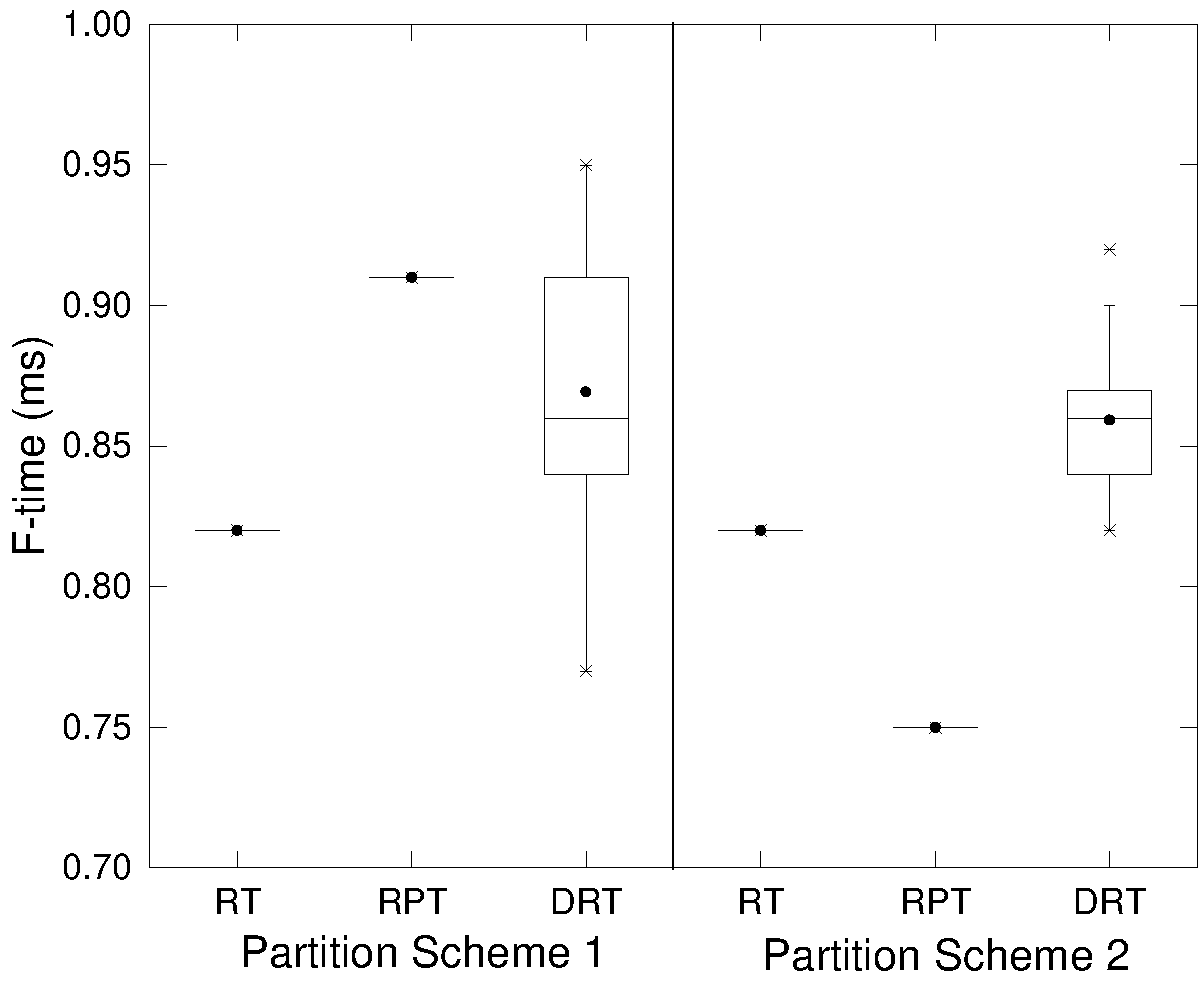
\includegraphics[width=0.32\textwidth,height=4cm]{fig/drttime/chinatimef}}
	\subfigure[PBS] {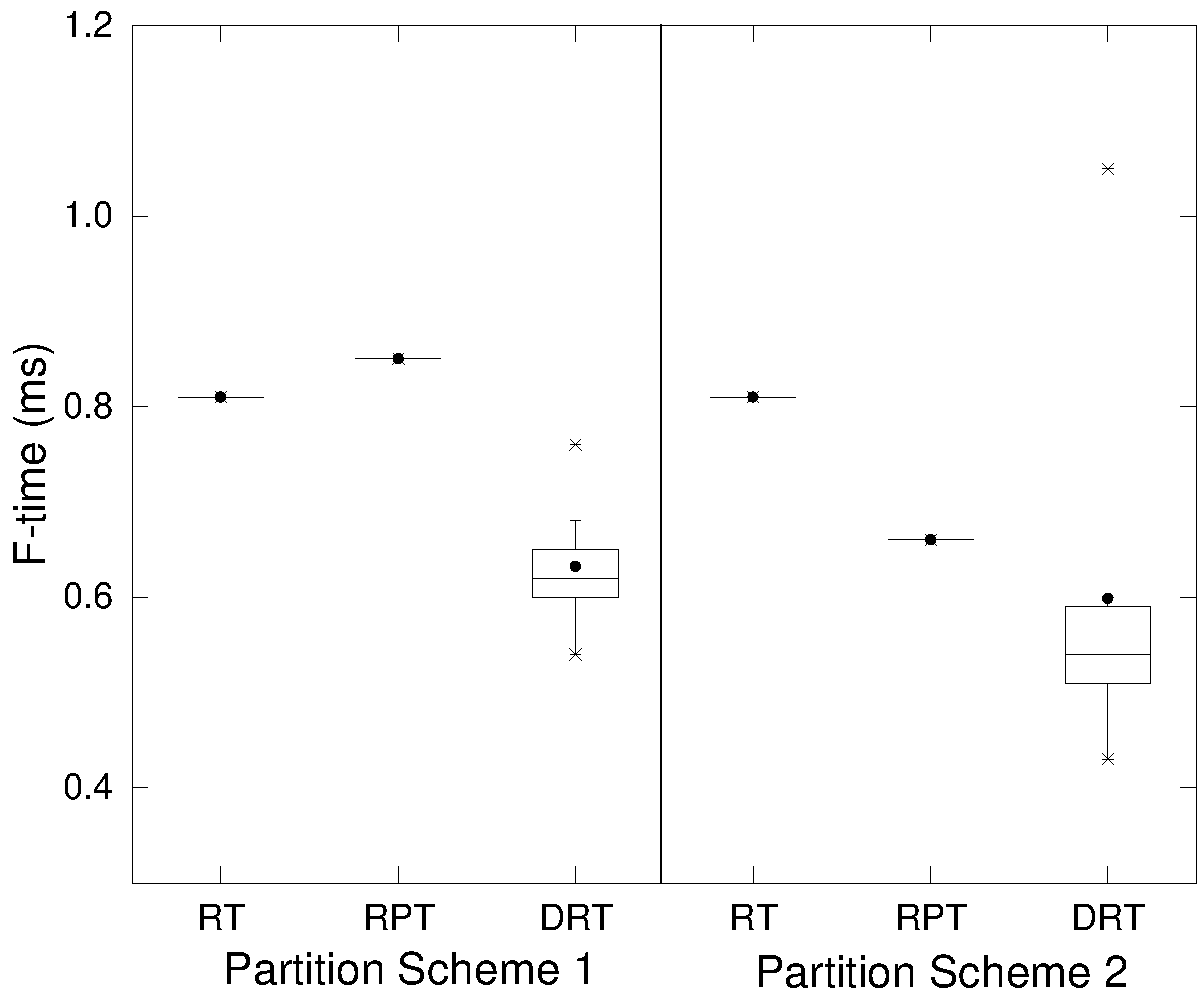
\includegraphics[width=0.32\textwidth,height=4cm]{fig/drttime/parkingtimef}}
	\caption{F-time boxplots for each program}
	\label{fig:Ftime}
\end{figure*}

\begin{figure*}
	\centering
	\subfigure[ACMS] {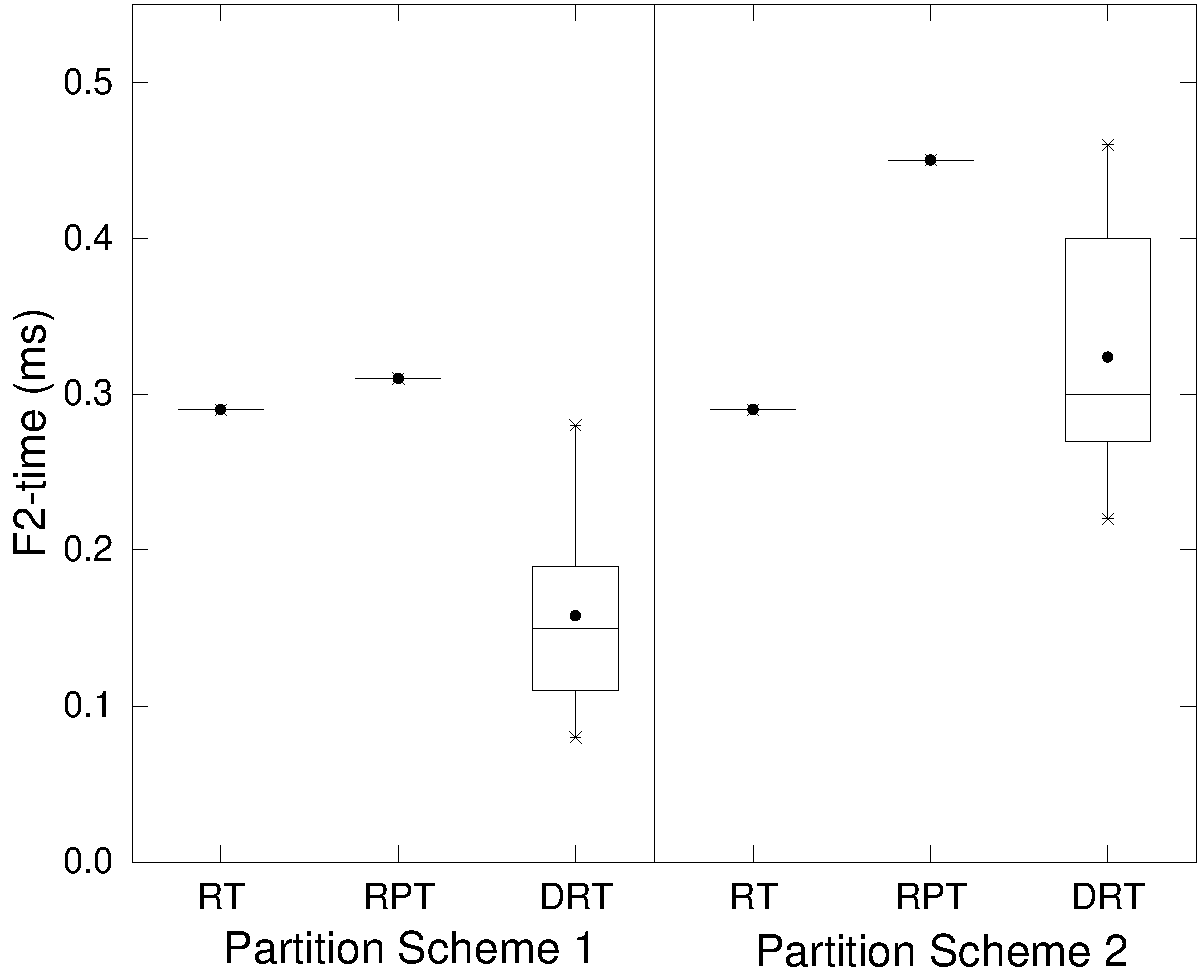
\includegraphics[width=0.32\textwidth,height=4cm]{fig/drttime/aviatimef2}}
	\subfigure[CUBS] {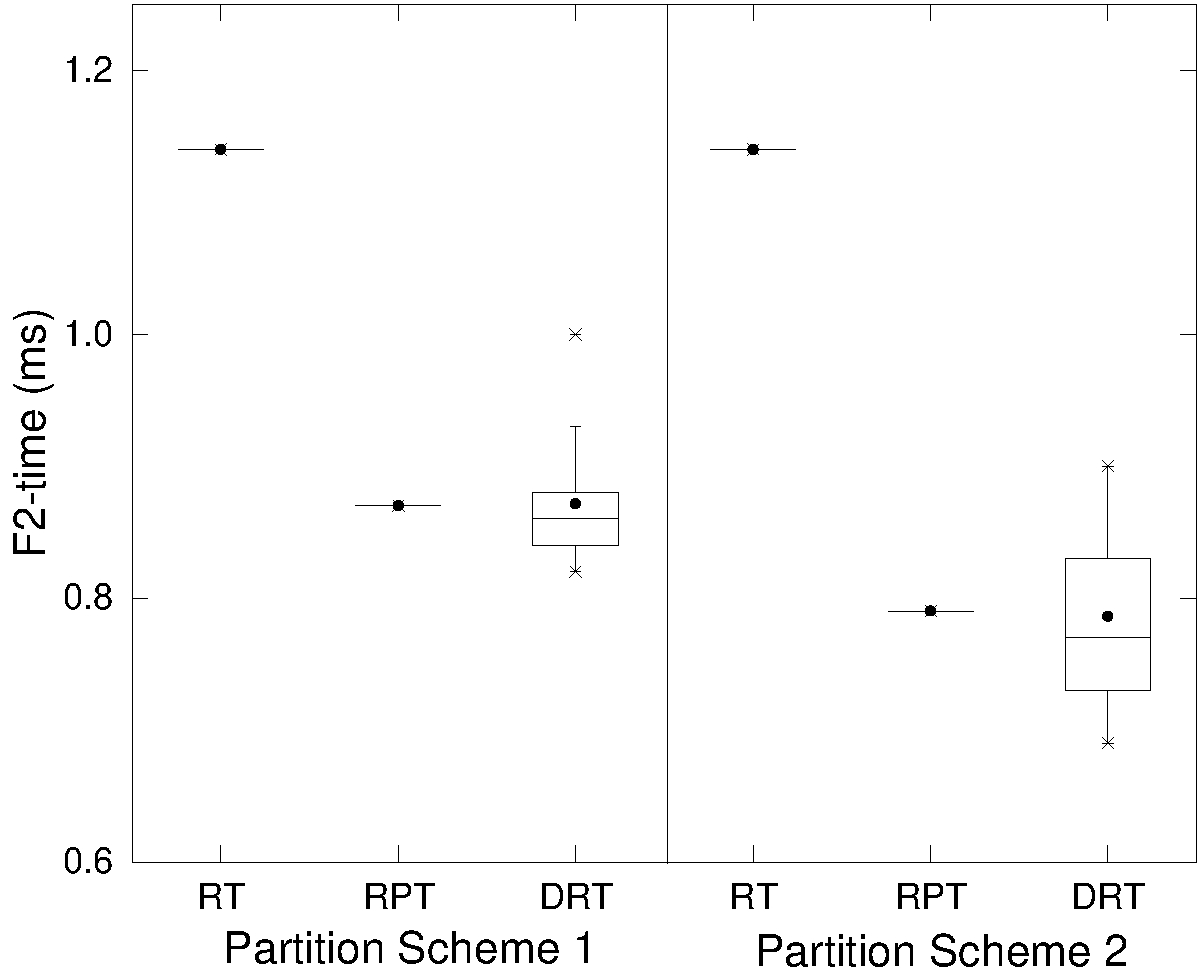
\includegraphics[width=0.32\textwidth,height=4cm]{fig/drttime/chinatimef2}}
	\subfigure[PBS] {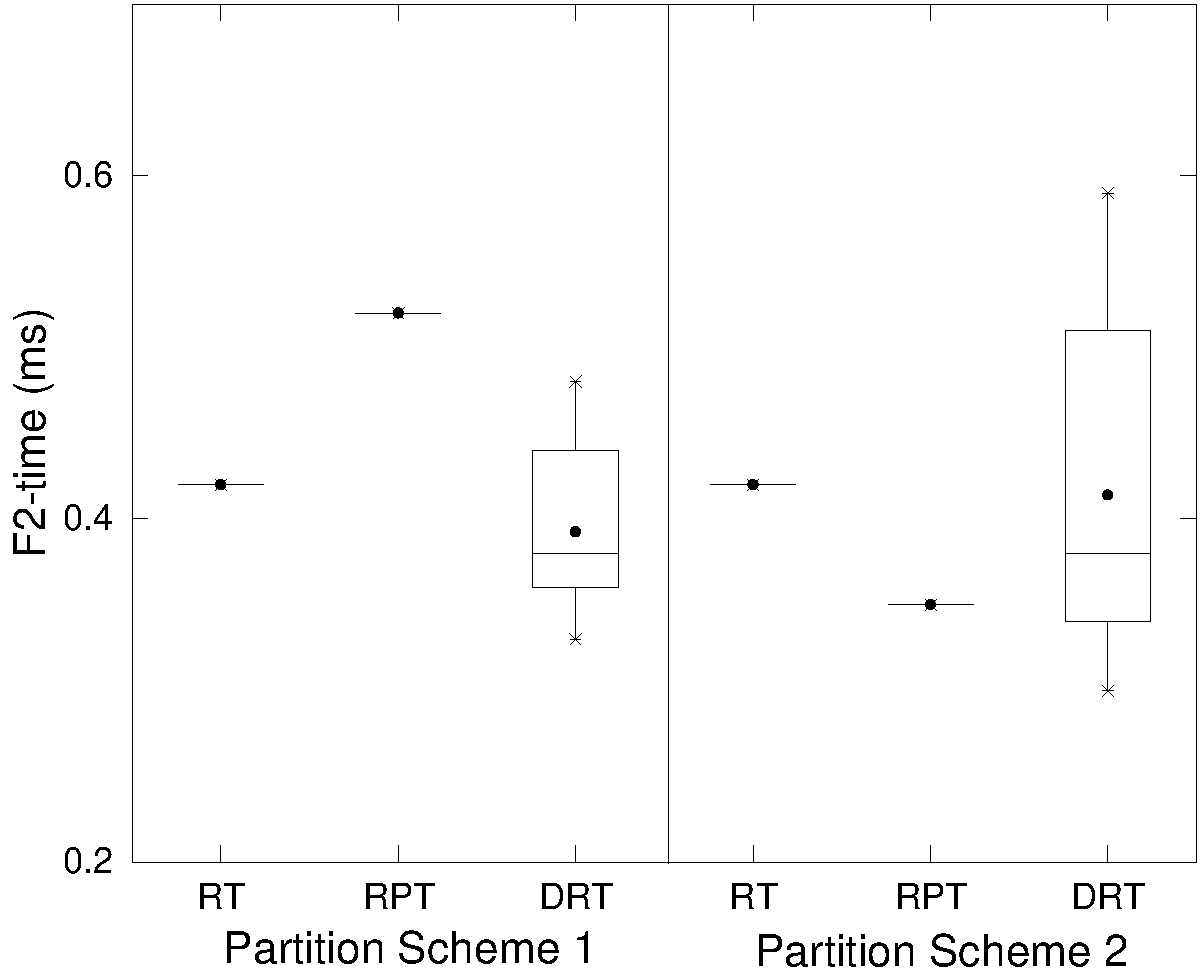
\includegraphics[width=0.32\textwidth,height=4cm]{fig/drttime/parkingtimef2}}
	\caption{F2-time boxplots for each program}
	\label{fig:F2time}
\end{figure*}


\begin{figure*}
	\centering
	\subfigure[ACMS] {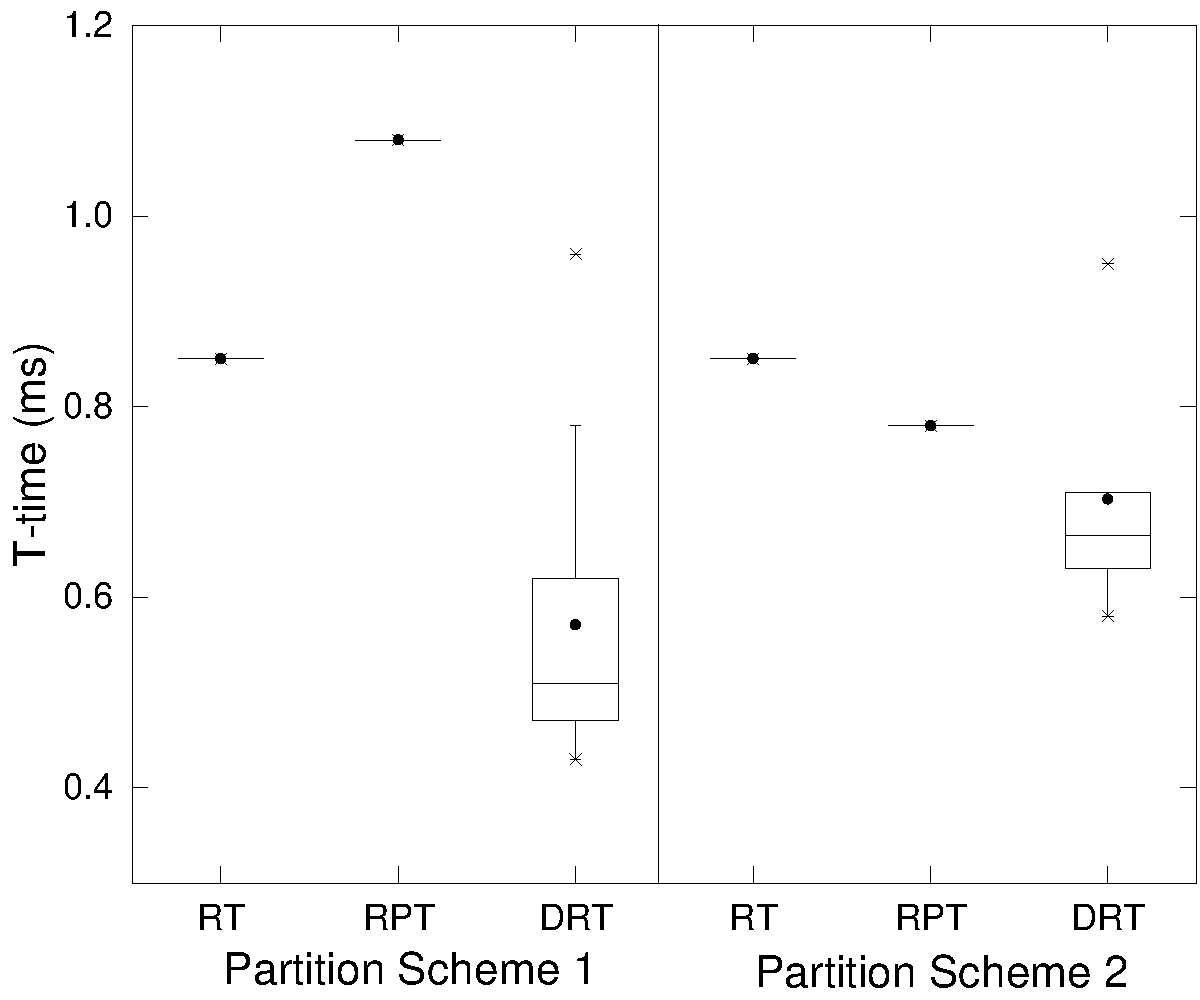
\includegraphics[width=0.32\textwidth,height=4cm]{fig/drttime/aviatimet}}
	\subfigure[CUBS] {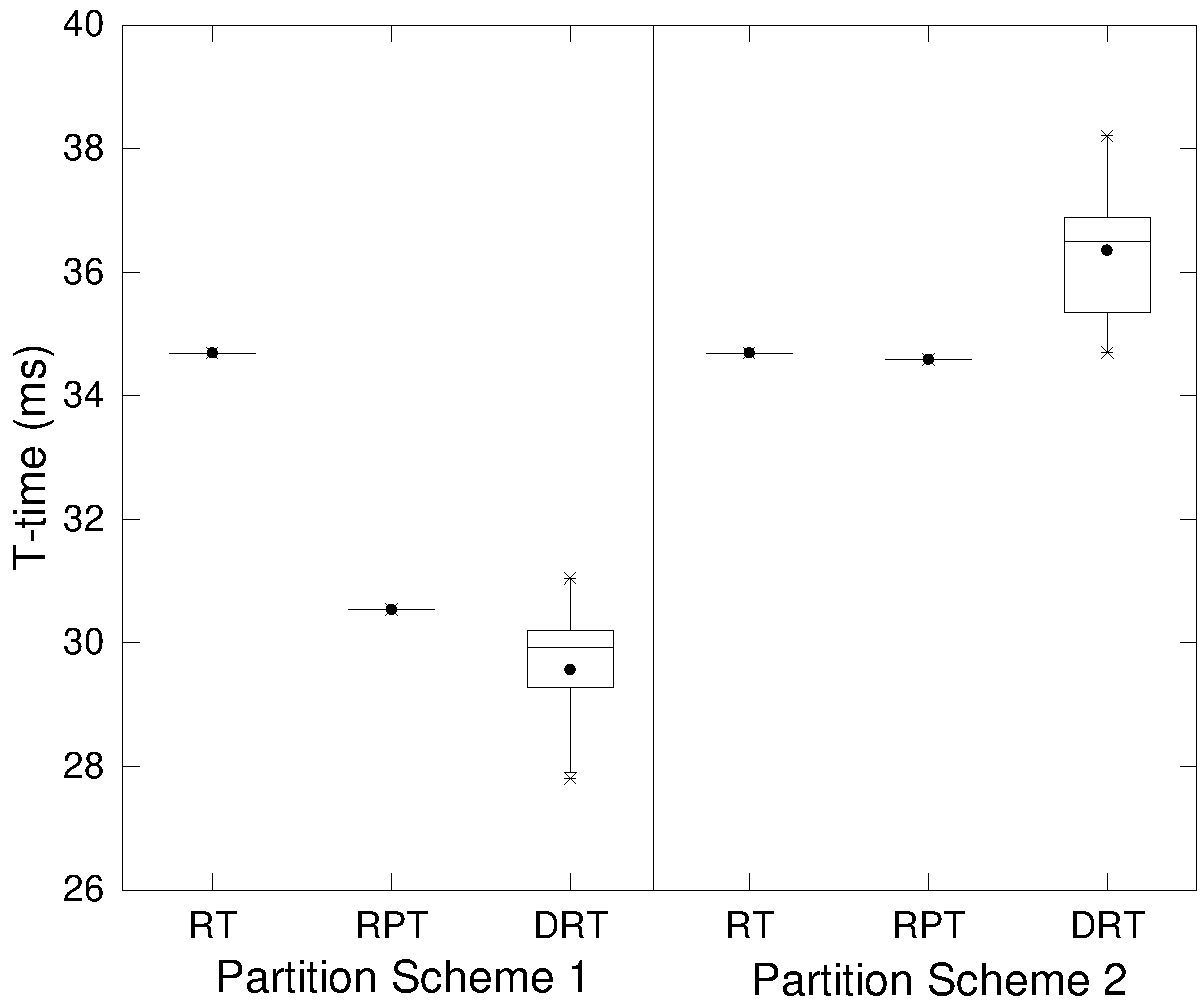
\includegraphics[width=0.32\textwidth,height=4cm]{fig/drttime/chinatimet}}
	\subfigure[PBS] {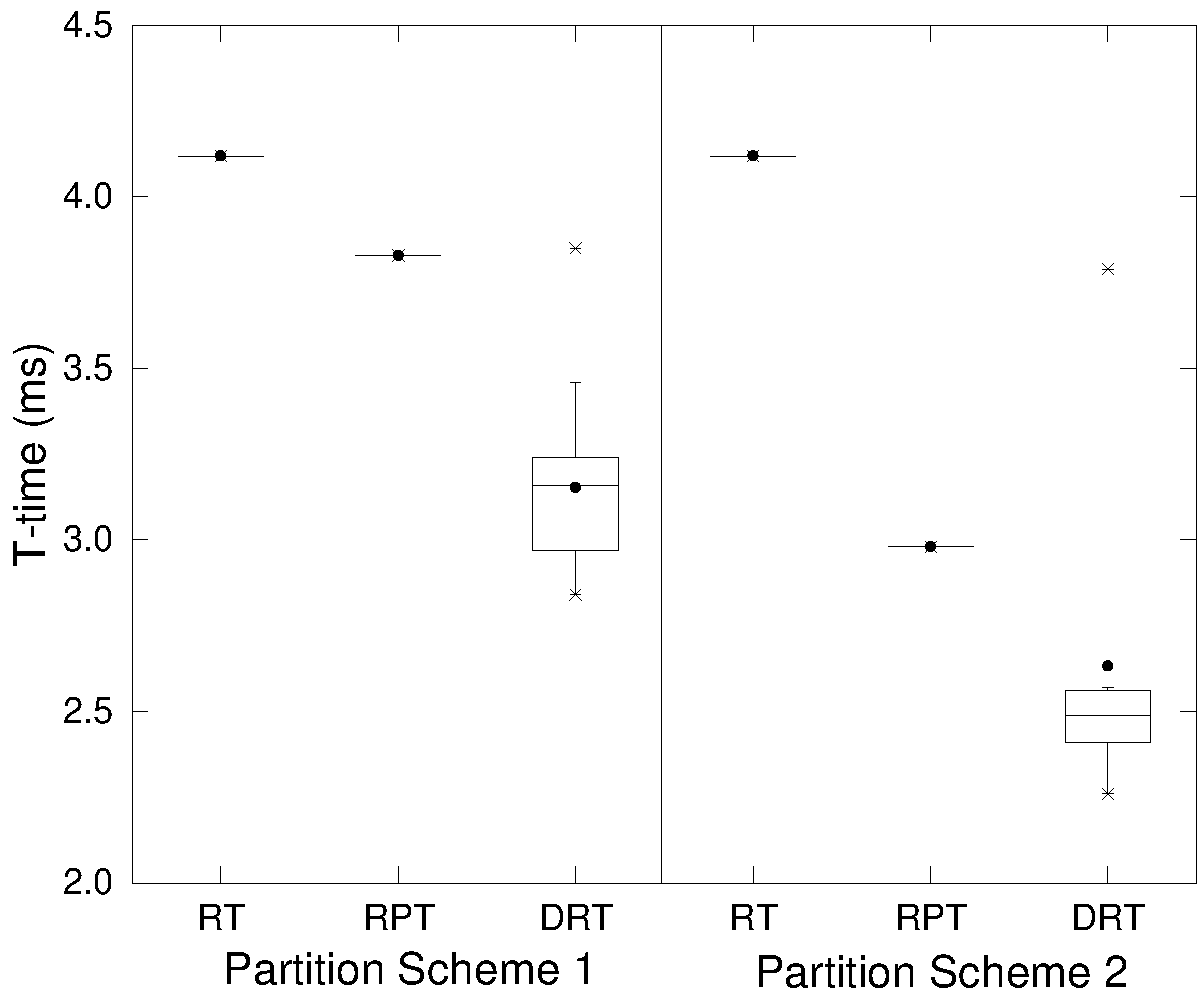
\includegraphics[width=0.32\textwidth,height=4cm]{fig/drttime/parkingtimet}}
	\caption{T-time boxplots for each program}
	\label{fig:Ttime}
\end{figure*}

As was done for the F-, F2-, and T-measure data, we used the Holm-Bonferroni method to check the difference between each pair of testing strategies in terms of F-time, F2-time, and T-time, as shown in Table \ref{tableHlom:f/f2/t-time}.

In Table \ref{tableHlom:f/f2/t-time}, some entries (such as "\underline{\textbf{61}}" \& "\underline{\textbf{17}}" for DRT vs. RT, "\underline{\textbf{57}}" vs. "\underline{\textbf{21}}" for DRT vs. RPT) are in bold font and underline, meaning that, in terms of F-/F2-/T-time, DRT was significantly better than RT, and DRT only marginally outperformed RPT.
In other words, the additional computation incurred in DRT by updating the test profile is compensated for in terms of test execution savings.

\begin{table}[htbp]
  \caption{Number of Scenarios Where the Technique on the Top Wow Has a Lower Metric (F-/F2/T-time) Score Than That on The Left Column}
  \centering
  \label{tableHlom:f/f2/t-time}
  \begin{tabular}{|c|c|c|c|c|c|c|c|c|c|}  \hline
  \multirow{2}{*}{}  &\multicolumn{3}{|c|}{F-measure}                  &\multicolumn{3}{|c|}{F2-measure}        &\multicolumn{3}{|c|}{T-measure} \\ \cline{2-10}
                     & \!RT\!    &  \!RPT\!    &\!DRT\!                & \!RT\!    &  \!RPT\!    &\!DRT\!       & \!RT\!    &  \!RPT\!    &\!DRT\!          \\ \hline
  RT                 & ---   &5        &\underline{\textbf{53}}        & ---   &3     &\underline{\textbf{62}}  & ---   &5   &\underline{\textbf{61}}  \\ \hline
  RPT                &1      & ---     &\underline{\textbf{59}}        &3      & ---  &\underline{\textbf{57}}  &1      &---     &\underline{\textbf{57}} \\ \hline
  DRT&\underline{\textbf{25}}&\underline{\textbf{19}}&---&\underline{\textbf{16}} &\underline{\textbf{21}} &--- &\underline{\textbf{17}}  &\underline{\textbf{21}} & ---  \\ \hline
  \end{tabular}
\end{table}

It can also be observed from Table~\ref{tableHlom:f/f2/t-time} that DRT only slightly outperformed RPT, but that DRT was significantly better than RT, especially in term of $T$-$time$.

In summary, the DRT strategy is considered the best testing technique across all six metrics, and RPT marginally outperformed RT.

\section{Related Work}
\label{sec:relatedwork}

In this section, we describe related work from two perspectives:
related to testing techniques for web services; and
related to improving RT and PT.

\subsection{Testing Techniques for Web Services}
\label{sec:relatedworkWS}

In recent years, a lot of effort has been made to test web services~\cite{canfora, bozkurt2010, li2014two, qiu2015regression}.
Test case generation or selection is core to testing web services, and model-based~\cite{dalal1999model} and specification-based~\cite{li2009towards} techniques are two common approaches.
Before making services available on the Internet, testers can use model-based techniques to verify whether or not the behavior of the WSUT meets their requirements.
In these techniques, test data can be generated from a data model that specifies the inputs to the software---this data model can be built before, or in parallel to, the software development process.
Verification methods using technologies such as theorem-proving~\cite{sinha2006model}, models~\cite{paradkar2007} and Petri-Nets~\cite{xiang2015executable} also exist.

All the above approaches aim to generate test cases without considering the impact of test case execution order on test efficiency.
In contrast, Bertolino et al.~\cite{bertolino2007automatic} proposed using the category-partition method~\cite{Ostrand88} with XML schemas to perform XML-based partition testing.
Because PT aims to find subsets of all possible test cases to adequately test a system, it can help reduce the required number of test cases.
Our approach involved software cybernetics and PT:
In DRT, selection of a partition is done according to the testing profile, which is updated throughout the test process.
An advantage of DRT is that partitions with larger failure rates have higher probabilities of selection.
Zhu and Zhang~\cite{zhu2012collaborative} proposed a collaborative testing framework, where test tasks are completed using collaborating test services---a test service is a service assigned to perform a specific testing task.
Our framework (Section~\ref{sec:framework}) aims to find more faults in the WSUT, with the result of the current test case execution providing feedback to the control system so that the next test case selected has a greater chance to reveal faults.

Most web service testing techniques assume that the computed output for any test case is verifiable, which is however not always true in practice (known as the oracle problem \cite{barr2015oracle, patel2018mapping}). Thus, many testing techniques may not be applicable in some cases.
To address the common oracle problem for testing web services, a metamorphic testing~\cite{chen1998metamorphic,chen2018metamorphic} approach has been proposed that not only alleviates the oracle problem, but also presents a feasible and efficient option for testing web services.
Sun et al. proposed a metamorphic testing framework for web services~\cite{sun2011} and conducted a case study that showed that up to 94.1\% of seeded faults could be detected without the need for oracles.

\subsection{Improving RT and PT}
\label{sec:relatedworkRT}

Based on the observation that failure-causing inputs tend to cluster into contiguous regions in the input domain~\cite{Ammann88, Finelli91}, many works have been done to improve RT~\cite{cai2009random, chen2010adaptive}.
Adaptive random testing~\cite{chen2010adaptive} is a family of techniques based on random testing that aim to improve the failure-detection effectiveness by evenly spreading test cases throughout the input domain.
One well-known ART approach, FSCS-ART, selects a next test input from the fixed-size candidate set of tests that is farthest from all previously executed tests~\cite{chen2004adaptive}.
Many other ART algorithms have also been proposed, including RRT \cite{chan2002restricted, chan2006restricted}, DF-FSCS \cite{mao2017out}, and ARTsum \cite{barus2016cost}, with their effectiveness examined and  validated through simulations and experiments.

Adaptive testing (AT) \cite{Cai07, hu2005case, hu2009improved} takes advantage of feedback information to control the execution process, and has been shown to outperforms RT and RPT in terms of the T-measure and the number of detected faults, which means that AT has higher efficiency and effectiveness than RT and RPT.
However, AT may require a very long execution time in practice.
To alleviate this, Cai et al.~\cite{cai2009random} proposed DRT, which uses testing information to dynamically adjust the testing profile.
There are several things that can impact on DRT's test efficiency.
Yang et al.~\cite{Yang2014Dynamic} proposed A-DRT, which adjusts parameters during the testing process.

\section{Conclusion}
\label{sec:conclusion}

In this paper, to address the challenges of testing SOA-based applications, we have presented a dynamic random testing (DRT) method for web services.
Our method uses random testing to generate test cases, and selects test cases from different partitions in accordance with a testing profile that is dynamically updated in response to the test data collected.
In this way, the proposed method includes enjoys benefits from both random testing and partition testing.

We proposed a framework that examines key issues when applying DRT to test web services, and developed a prototype to make the method  feasible and effective.
To guide testers to correctly set the DRT parameters, we used a theoretical analysis to study the relationships between the number of partitions ($m$) and the probability adjusting factor ($\varepsilon$).
Three real web services were used as experimental subjects to validate the feasibility and effectiveness of our approach.
Our experimental results show that, in general, DRT has better performance than both RT and RPT, in terms of the F-, F2-, and T-measures, and always outperforms when the $\varepsilon$ settings follow our guidelines.
In other words, our theoretical analysis can provide genuinely useful guidance to use DRT.

In our future work, we plan to conduct experiments on more web services to further validate its effectiveness, and identify the limitations of our method.

\section*{Acknowledgment}

This research is supported by
the National Natural Science Foundation of China (Grant Nos. 61872039 and 61872167),
the Beijing Natural Science Foundation (Grant No. 4162040),
the Aeronautical Science Foundation of China (Grant No. 2016ZD74004), and
the Fundamental Research Funds for the Central Universities (Grant No. FRF-GF-17-B29).
\ifCLASSOPTIONcaptionsoff
  \newpage
\fi
\bibliographystyle{IEEEtran}
\bibliography{DRT4WS}
\vspace{-10ex}
\begin{IEEEbiography}[{
\includegraphics[width=1in,height=1.25in,clip,keepaspectratio]{fig/authors/CASun.pdf}}]{Chang-ai Sun} is a Professor in the School of Computer and Communication Engineering, University of Science and Technology Beijing.
Before that, he was an Assistant Professor at Beijing Jiaotong University, China, a postdoctoral fellow at the Swinburne University of Technology, Australia, and a postdoctoral fellow at the University of Groningen, The Netherlands. He received the bachelor degree in Computer Science from the University of Science and Technology Beijing, China, and the PhD degree in Computer Science from Beihang University, China.
His research interests include software testing, program analysis, and Service-Oriented Computing.
\end{IEEEbiography}
\vspace{-10ex}
\begin{IEEEbiography}[{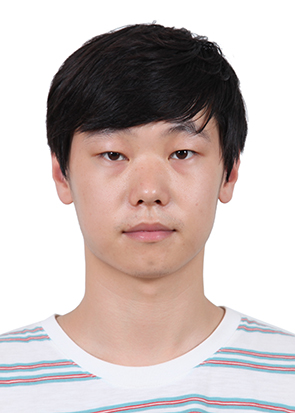
\includegraphics[width=1in,height=1.25in,clip,keepaspectratio]{fig/authors/HPDai.jpg}}]{Hepeng Dai} is a PhD student in the School of Computer and Communication Engineering, University of Science and Technology Beijing, China. He received the master degree in Software Engineering from University of Science and Technology Beijing, China and the bachelor degree in Information and Computing Sciences from China University of Mining and Technology, China. His current research interests include software testing and debugging.
\end{IEEEbiography}
\vspace{-10ex}
\begin{IEEEbiography}[{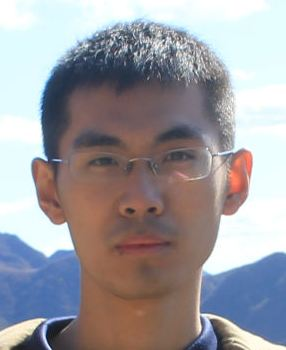
\includegraphics[width=1in,height=1.25in,clip,keepaspectratio]{fig/authors/GWang.jpg}}]{Guan Wang} is a masters student at the School of Computer and Communication Engineering, University of Science and Technology Beijing. He received a bachelor degree in Computer Science from University of Science and Technology Beijing. His current research interests include software testing and Service-Oriented Computing.
\end{IEEEbiography}
\vspace{-10ex}
\begin{IEEEbiography}[{
\includegraphics[width=1in,height=1.25in,clip,keepaspectratio]{fig/authors/DaveTowey.png}}]{Dave Towey} is an associate professor in the School of Computer Science, University of Nottingham Ningbo China. He received his BA and MA degrees from The University of Dublin, Trinity College, PgCertTESOL from The Open University of Hong Kong, MEd from The University of Bristol, and PhD from The University of Hong Kong. His current research interests include technology-enhanced teaching and learning, and software testing, especially metamorphic testing and adaptive random testing. He is a  member of both the IEEE and the ACM.
\end{IEEEbiography}
\vspace{-10ex}
\begin{IEEEbiography}[{
\includegraphics[width=1in,height=1.25in,clip,keepaspectratio]{fig/authors/TYChen.pdf}}]{Tsong Yueh Chen} is a Professor of Software Engineering at the Department of Computer Science and Software Engineering in Swinburne University of Technology. He received his PhD in Computer Science from The University of Melbourne, the MSc and DIC from Imperial College of Science and Technology, and BSc and MPhil from The University of Hong Kong. He is the inventor of metamorphic testing and adaptive random testing.
\end{IEEEbiography}
\vspace{-10ex}
\begin{IEEEbiography}[{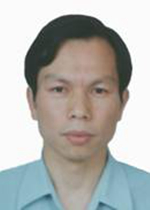
\includegraphics[width=1in,height=1.25in,clip,keepaspectratio]{fig/authors/KYCai.pdf}}]{Kai-Yuan Cai} received the BS, MS, and PhD degrees from Beihang university, Beijing, China, in 1984, 1987, and 1991, respectively. He has been a full professor at Beihang University since 1995. He is a Cheung Kong Scholar (chair professor), jointly appointed by the Ministry of Education of China and the Li Ka Shing Foundation of Hong Kong in 1999. His main research interests include software testing, software reliability, reliable flight control, and software cybernatics.
\end{IEEEbiography}

\end{document}
